\documentclass[12pt,a4paper]{report}
\usepackage{dissertation}
\makeglossaries
\makeindex

%\logo{EAAD}{Escola de Arquitetura, Arte e Design}{}
%\logoB{EAAD}{Escola de Arquitetura, Arte e Design}{}

%\logo{EC}{Escola de Ciências}{}
%\logoB{EC}{Escola de Ciências}{}

%\logo{ED}{Escola de Direito}{}
%\logoB{ED}{Escola de Direito}{}

\logo{EE}{Escola de Engenharia}{}
\logoB{EE}{Escola de Engenharia}{}

%\logo{EEG}{Escola de Economia e Gestão}{}
%\logoB{EEG}{SEscola de Economia e Gestão}{}

%\logo{ELACH}{Escola de Letras, Artes e Ciências Humanas}{}
%\logoB{ELACH}{Escola de Letras, Artes e Ciências Humanas}{}

%\logo{EM}{Escola de Medicina}{}
%\logoB{EM}{Escola de Medicina}{}

%\logo{EP}{Escola de Psicologia}{}
%\logoB{EP}{Escola de Psicologia}{}

%\logo{ESE}{Escola Superior de Enfermagem}{}
%\logoB{ESE}{Escola Superior de Enfermagem}{}

%\logo{I3Bs}{Instituto de Investigação em Biomateriais,}{Biodegradáveis e Biomiméticos}
%\logoB{I3Bs}{Instituto de Investigação em Biomateriais,}{Biodegradáveis e Biomiméticos}

%\logo{ICS}{Instituto de Ciências Sociais}{}
%\logoB{ICS}{Instituto de Ciências Sociais}{}

%\logo{IE}{Instituto de Educação}{}
%\logoB{IE}{Instituto de Educação}{}

\author{Nome completo do autor}

\titleA{Título Título Título Título Título Título}
\titleB{Título Título Título Título Título}
\titleC{Título Título Título Título}

\masters{Mestrado em Engenharia Informática}
%\area{Área de especialização}
\supervisor{Nome do Orientador}
\cosupervisor{Nome do Coorientador}

\begin{document}
\setlength{\parindent}{0em}

%-- Covers
\begin{titlepage}
\color{PANTONECoolGray7C}
\thelogo
\leading{20.4pt}
{\Large
\theauthor
\\
%
\\
\textbf{\thetitleA}
\\
\textbf{\thetitleB}
\\
\textbf{\thetitleC}
}

\vspace*{\fill}
{\footnotesize \myear}
\end{titlepage}

\null
\thispagestyle{empty}
\pagecolor{PANTONECoolGray7C}
\afterpage{\nopagecolor}
\newpage

\begin{titlepage}
\color{PANTONECoolGray7C}
\thelogoB
\leading{20.4pt}
{\Large
\theauthor
\\
%
\\
\textbf{\thetitleA}
\\
\textbf{\thetitleB}
\\
\textbf{\thetitleC}
}

\vspace{55.2mm}
\leading{16.8pt}
{\large
Dissertação de Mestrado
\\
\themasters
\\
\thearea
Trabalho efetuado sob a orientação de
\\
\textbf{\thesupervisor}
\\
\thecosupervisor}

\vspace*{\fill}
{\footnotesize \myear}
\end{titlepage}

%-- Document setup
\newgeometry{right=25mm, left=25mm, top=25mm, bottom=25mm}
\pagenumbering{roman}

\setlength{\parskip}{0pt}
\setlength{\parindent}{1.5em}

%-- Preamble
\chapter*{Direitos de Autor e Condições de Utilização do Trabalho por Terceiros}
\setlength{\parskip}{1em}
\noindent
Este é um trabalho académico que pode ser utilizado por terceiros desde que respeitadas as regras e boas práticas internacionalmente aceites, no que concerne aos direitos de autor e direitos conexos.

\noindent
Assim, o presente trabalho pode ser utilizado nos termos previstos na licença abaixo indicada.

\noindent
Caso o utilizador necessite de permissão para poder fazer um uso do trabalho em condições não previstas no licenciamento indicado, deverá contactar o autor, através do RepositóriUM da Universidade do Minho.

\section*{Licença concedida aos utilizadores deste trabalho:}



%--

\noindent

\includegraphics[]{images/CCBYNCSA.png}
\\
\textbf{CC BY-NC-SA}
\\
\url{https://creativecommons.org/licenses/by-nc-sa/4.0/}

%--

\noindent

\setlength{\parskip}{0em}
\chapter*{Agradecimentos}
\setlength{\parskip}{1em}

Escreva aqui os seus agradecimentos. Não se esqueça de mencionar, caso seja esse o caso, os projetos e bolsas dos quais se beneficiou enquanto fazia a sua investigação. Pergunte ao seu orientador sobre o formato específico a ser usado. (As agências de financiamento são bastante rigorosas quanto a isso.)

\setlength{\parskip}{0em}
\chapter*{Declaração de Integridade}
\setlength{\parskip}{1em}
\noindent
Declaro ter atuado com integridade na elaboração do presente trabalho académico e confirmo que não recorri à prática de plágio nem a qualquer forma de utilização indevida ou falsificação de informações ou resultados em nenhuma das etapas conducente à sua elaboração.

\noindent
Mais declaro que conheço e que respeitei o Código de Conduta Ética da Universidade do Minho.


\phantom{space for signature}

\noindent
Universidade do Minho, Braga, \myear

\vspace{25mm}
\noindent\theauthor
\setlength{\parskip}{0em}
\chapter*{Resumo}

\newacronym{ocr}{OCR}{reconhecimento óptico de caracteres}
\newacronym{gui}{GUI}{graphic user interface}

A digitalização de documentos permitiu uma nova forma de salvaguardar informação para a posteridade, evitando a sua perda pelo deterioramento físico destes. De forma a posteriormente transcrever estes documentos, permitindo uma consulta, processamento e manipulação mais simples, o uso de software de \acrshort{ocr} é essencial. Esta tecnologia é, no entanto, dependente em diferentes níveis das características do seu alvo, nomeadamente: qualidade da imagem, complexidade da estrutura do documento, linguagem do texto. 

Documentos mais antigos, em especial jornais por apresentarem estruturas mais complexas, apresentam por este motivo resultados que diferem bastante do seu conteúdo original; tanto a nível do texto reconhecido, como da sua organização para os diferentes outputs disponíveis (ex.: txt simples). A tarefa de extrair informação destes documentos, como por exemplo o isolamento e extração de artigos, torna-se assim complexa e propensa a erros. 

Este trabalho propõe então a criação de uma ferramenta ou um conjunto de ferramentas que permitam auxiliar o processo de extração de conteúdo de documentos, primeiramente mas não exclusivamente, mais antigos e estruturados, com especial foco em jornais. A pipeline do projeto pretende então ser capaz de detetar e lidar com os diferentes pontos de risco nestes documentos: qualidade da imagem, erros nos resultados de \acrshort{ocr}, segmentação e organização do documento, criação do output organizado. 

Diferentes alternativas para \acrshort{ocr} assim como métodos de tratamento destes problemas serão estudados, comparados, e implementados, de forma a encontrar a melhor solução para a resolução deste problema. O produto final implementado será composto por uma ferramenta utilizável num formato \acrshort{gui} ou comando de consola. 

Para documentos antigos a linguagem, como mencionado, pode afetar os resultados de \acrshort{ocr}. Deste modo, como objetivo secundário, propõe-se a criação de uma ferramenta que facilite a criação de um dicionário para diferentes iterações de uma linguagem para: fornecer ao motor \acrshort{ocr} um léxico mais apropriado; modernizar o conteúdo extraído.

\paragraph{Palavras-chave} OCR, Digitalização, Documentos estruturados, Documentos antigos, Segmentação de documentos, Tratamento de imagem, Modernização de texto

\cleardoublepage

\chapter*{Abstract}

The digitization of documents has opened a new way of preserving information for posterity, avoiding its loss through their physical decay. To allow the transcription of these documents, enabling an easier search, indexation and manipulation of them, the use of \acrshort{ocr} software is essential. This technology is, however, dependent in many ways of the characteristics of its target, namely: the quality of the image, the complexity of the document's structure, the text's language. 

Older documents, especially newspapers for having complex structures, result in poor transcriptions that differ from their original content, both in the recognized text, and in the organization of the available final outputs (ex.: simple txt).
Extracting information from these documents, for example, the isolation and extraction of articles, becomes thus a complex and error prone task. 

Therefore, this work aims to create a tool, or a toolkit, that can assist in the process of content extraction from documents, primarily though not exclusively, that are older and structured, specializing in newspapers. The proposed pipeline should then be able to detect and fix potential problems in these documents: image quality, \acrshort{ocr} results errors, segmentation and document organization, restructured output generation.

Different \acrshort{ocr} alternatives, as well as different methods of dealing with these problems, will be studied, compared, and implemented, to find the best solution for the task at hand. The final product will be composed of a tool usable in both a \acrshort{gui} and bash command format.

For old documents, its language, as mentioned, may affect the \acrshort{ocr}'s performance. Therefore, as a secondary objective, it’s proposed the development of a tool that allows for the creation of dictionaries for different versions of a given language that can be used to: supply the \acrshort{ocr} engine with a more appropriate lexicon; modernize the extracted content.


\paragraph{Keywords} OCR, Digitalization, Structured documents, Old documents, Document segmentation, Image treatment, Text modernization

\cleardoublepage


\phantomsection
\tableofcontents

\cleardoublepage
\listoffigures

% List of tables
\listoftables
\clearpage

% Acronyms
\printglossary[type=\acronymtype,nonumberlist, title={Acrónimos}]

% Glossary
\printglossary[title={Glossário}, nonumberlist]

\cleardoublepage
\pagenumbering{arabic}

%-- Dissertation 
\part{Material Introdutório}

\chapter{Introdução}
\label{cap_introducao}

Neste capítulo, será realizada uma introdução ao problema que o projeto tenciona abordar, composta por uma contextualização do seu estado atual e os desafios que sobre este são impostos. Além disso, os objetivos do trabalho serão listados e será descrita a estrutura do documento.

%Contexto, motivação, principais objetivos.
\section{Enquadramento e motivação}


A digitalização tem um papel fundamental na conservação, disponibilização e proliferação de documentos físicos, não só contemporâneos, mas também de eras anteriores à revolução da informação. Esta tecnologia, acoplada a ferramentas de \acrshort{ocr}, veio trazer uma facilidade de navegação, consulta e manipulação destes documentos que anteriormente não era possível.

A eficácia de \acrshort{ocr} é no entanto dependente de vários fatores nas imagens ou ficheiros alvo: a qualidade das imagens, como a resolução, estado do documento, coloração, qualidade/tipo de escrita; a estrutura dos documentos - quanto mais complexo, mais difícil é obter a informação de forma automática mantendo 
 a congruência original -; linguagem do texto, sendo que por vezes diferentes tecnologias, como por exemplo \textbf{Tesseract}, procuram verificar a sua confiança na deteção com o vocabulário conhecido, o qual pode não coincidir com a época de produção do documento; entre outras. 

Estas dependências são especialmente notórias quando se envolvem documentos mais antigos, os quais podem, além de apresentar envelhecimento causado pelo tempo e danos pelas condições de armazenamento, devido às limitações tecnológicas assim como por vezes à falta de convenções de formatação dos documentos, não dispor de uma consistência no formato e texto (estrutura, alinhamento, dimensões dos caracteres, fonte de texto consistente, etc.) usual nos documentos atuais. Estes fatores resultam então num reconhecimento de texto não tão satisfatórios. 

Estes documentos antigos são mais comummente, mas não exclusivamente, reconhecidos como anteriores à era digital, sendo que o foco de trabalho será maioritariamente dirigido a documentos desta época, como jornais, revistas e outros, do século passado ou anteriores. 
Em especial documentos com estruturas complexas, como é o caso de jornais, onde é possível a segmentação em diferentes partes com conteúdo e propósito distinto e, ao mesmo tempo, uma ordem de leitura complexa i.e., não segue apenas regras simples de posição do conteúdo (texto da esquerda antes do texto da direita e cima antes de baixo), exigindo também noção das características e relação do conteúdo. 

Mesmo para ficheiros do tipo \textbf{hOCR} ou \textbf{PDF}, que já passaram por um processo de reconhecimento de texto, a complexidade da estrutura dos documentos originais ou problemas nos elementos que contém o texto (como por exemplo elementos sobrepostos ou que se intersetam) dificultam a extração e interpretação do seu conteúdo, podendo ser facilmente perdida a lógica original.

Por estas razões, seria útil uma ferramenta que permita uma deteção e tratamento destes documentos de forma automática e de uso simples, permitindo um certo nível de configuração para adaptação entre tipos de documentos com características bem definidas e distintas. 

O presente documento pretende então servir como um estudo dos desafios apresentados por estes tipos de documentos perante \acrshort{ocr}, assim como a procura de soluções para a melhoria dos resultados na deteção  e extração de texto e assim criar uma ferramenta que torne o processo de extração de informação destes tipos de documentos mais simples e fiável. 

Como trabalho complementar, é proposta a implementação de um método de modernização do conteúdo extraído, envolvendo a criação de uma ferramenta capaz de criar dicionários entre diferentes iterações de uma mesma linguagem. 

\section{Objetivos}
\label{section_objetivos}

O principal objetivo deste trabalho é a realização de um estudo sobre os problemas apresentados à extração de conteúdo de documentos de estrutura complexa - mantendo 
a sua lógica original -, assim como a implementação de uma solução para resolver ou mitigar estes desafios, aumentando a confiança na informação extraída. 
Em termos dos casos alvo do trabalho, será prioridade o estudo de jornais com texto máquina. Tal deve-se ao facto de jornais serem um particular tipo de documento que apresenta mais dificuldades e se encontra em maior procura de soluções e, texto máquina por ser mais comum para este tipo de documento. Esta segunda restrição é menos relevante pois não é uma dificuldade do trabalho e pode ser resolvida perante a escolha da tecnologia de reconhecimento utilizada.

Especificando, os objetivos do trabalho são:
\begin{itemize}
    \item Estudar os diferentes softwares de \acrshort{ocr} disponíveis e as diferenças entre estes.
    \item Estudar as dificuldades que documentos podem apresentar no processo de reconhecimento de texto.
    \item Estudar o trabalho desenvolvido sobre a área de tratamento de imagem, identificação de tipo de documento, segmentação de documentos, algoritmos de cálculo da ordem de leitura, melhoria de resultados de \acrshort{ocr} e métricas de validação de resultado \acrshort{ocr}.
    \item Estudar trabalhos com âmbito similar ou relacionado ao presente.
    \item Implementação de um conjunto de ferramentas dirigidas à solução dos problemas propostos.
    \item Implementação de uma ferramenta em formato \acrshort{gui} e comando de consola que aplique uma pipeline cujo input seria um ficheiro - imagem, pdf, hOCR -, identifique e trate de problemas deste se necessário para melhorar os resultados de \acrshort{ocr} e, por fim, devolva um output que mantenha a lógica e conteúdo do documento original.
    \item Secundário : ferramenta para criação de dicionário de diferentes versões de uma linguagem para: modernização de texto; léxico de motor \acrshort{ocr}. Ferramenta tem como input duas versões de um documento na mesma linguagem mas iterações diferentes e dá como output um dicionário entre as versões.
    \begin{itemize}
        \item Estudo sobre criação de léxicos e alinhamento de documentos.
    \end{itemize}
\end{itemize}



\section{Estrutura da dissertação}

Esta dissertação segue a seguinte estrutura:

\begin{itemize}
    \item Capítulo \ref{cap_introducao}: Breve contextualização sobre o tema proposto, as dificuldades impostas por documentos estruturados e com digitalizações ou condições físicas degradadas, nos resultados \acrshort{ocr}, e a utilidade de uma ferramenta para o tratamento destas. Além disso foram listados os objetivos do trabalho.

    \item Capítulo \ref{cap_estado_arte}: Estudo sobre o estado da arte nos tópicos relacionados ao tema da dissertação, as suas dificuldades e soluções destas; estudo de trabalho anteriormente realizado com âmbito similar ao atual ou técnicas relevantes para a construção da solução do problema.

    \item Capítulo \ref{cap_problema}: Listagem dos diferentes problemas que a solução irá abranger e os desafios que estes apresentam. Apresentação do desenho da solução.

    \item Capítulo \ref{cap_contribuicao}: Descrição da solução e ferramentas implementadas.

    \item Capítulo \ref{cap_aplicacoes}: Apresentação e estudo dos resultados do trabalho realizado.

    \item Capítulo \ref{cap_conclusao}: Reflexão sobre o trabalho realizado, os resultados e a experiência obtida, assim como uma breve exploração de caminhos para trabalho futuro do projeto. 

    \item Capítulo \ref{cap_planeamento}: No último capítulo é explicado o plano de desenvolvimento da dissertação.
\end{itemize}

\chapter{Estado da arte}
\label{cap_estado_arte}

Neste capítulo, será feita uma exposição do estado da arte das tecnologias relacionadas com o tema ou relevantes para o projeto, assim como trabalhos relacionados, quer no mesmo tema ou envolvente - algoritmos relevantes para o desenvolvimento -, procurando plantar uma base para o trabalho realizado e futuro, entendendo o que já foi explorado e o que está para vir em alguns casos.
O capítulo começa com uma apresentação sobre \acrshort{ocr} que será a tecnologia pilar do trabalho (\ref{sec_ocr}), seguido por uma exploração de processos de melhoria dos resultados de reconhecimento usando pré (\ref{sec_pre_proc_ocr}) e pós processamento (\ref{sec_pos_proc_ocr}). Procede-se o tema de segmentação de documentos (\ref{sec_segmentacao_docs}), terminando com o estudo de trabalho relacionado (\ref{sec_trab_relacionado}).

% pequeno resumo dos temas que serão tratados


\section{Reconhecimento ótico de caracteres}
\label{sec_ocr}


\subsection{Introdução}

O reconhecimento ótico de caracteres é a tecnologia base do projeto proposto, estando presente em qualquer instância ou caso de estudo que será explorado, inclusive em exceções que não necessitam a aplicação de reconhecimento de caracteres, como ficheiros do género \textbf{hOCR},  pois estes já são um produto de \acrshort{ocr}.

Na sua essência e como o nome indica, software de reconhecimento ótico de caracteres permitem a deteção e transcrição de texto a partir de imagens, de forma automática e autónoma. Utilizando esta habilidade, abriu-se a possibilidade de tornar os documentos digitalizados ao longo do tempo numa fonte mais útil de informação: navegada, consultada e editada mais facilmente, visto estes serem na maioria dos casos, digitalizados na forma de imagens. A adição do conteúdo destes documentos através da sua transcrição, mesmo que apenas parcialmente correta, permite a adição de, por exemplo, meta-dados ou palavras chaves que auxiliam a sua indexação. 




\subsection{Breve história e evolução}

\cite{10.5555/1074100.1074664} e \cite{6993174} apresentam a história do reconhecimento ótico de caracteres desde a conceção do seu ideal no século XIX, como uma tecnologia para auxílio de pessoas com impedimentos na leitura, até aos pontos alcançados na última década onde até escrita humana se tornou num desafio, até certo ponto, conquistável.
As primeiras instâncias de reconhecimento óptico realizado por máquinas deu-se no final do séc. XIX, mais especificamente em 1870 por Charles R. Carey  com a criação de um scanner de retina, mas é necessário ir até meio do século seguinte e pela consequente evolução que decorreu nesta área, para a subárea de reconhecimento de caracteres começar a ver a sua comercialização com a invenção de David Shepard: GISMO, um sistema simples capaz de reconhecer texto .

A génese desta tecnologia começou num formato bastante limitado, sendo capaz apenas de reconhecer um conjunto muito limitado de caracteres de uma fonte específica a um ritmo de 1 caráter por minuto, isto em condições de input bem controladas (papel sem ruído, apenas com o texto a ser reconhecido). Esta é considerada por \cite{6993174} como a primeira geração de \acrshort{ocr}.

A segunda geração começa a dar os primeiros passos no processamento de escrita humana, como é exemplo o \textit{IBM 1287} na década de 60.

A terceira geração, nas décadas de 70 e 80, introduziu um maior foco no processamento da escrita humana e na capacidade de lidar com problemas na imagem original.

A quarta geração tornou-se capaz de tratar documentos complexos com misturas entre texto e imagens, assim como qualidades de inputs menos favoráveis, documentos com cor e mais precisão com texto manuscrito.

Atualmente com a evolução das técnicas de pré processamento, assim como os algoritmos de reconhecimento e a ascensão da inteligência artificial \citep{9183326}, a precisão e flexibilidade dos softwares de \acrshort{ocr} são capazes de, até em imagens de paisagens, segmentar e reconhecer texto localmente de forma automática e com pouco pré processamento. Além disso, embora o foco anteriormente era em software \acrshort{ocr} pago e dedicado a um tipo específico de documentos, a implementação de softwares mais geral e de uso aberto tem-se tornado mais vulgar.
Em algumas instâncias complexas - documento complexo e linguagem com caracteres fora do latim -, já existe tecnologia capaz de obter taxas de acerto acima dos 95\% mesmo para texto escrito à mão \citep{9183326}.   


\subsection{Processo OCR}
Um software \acrshort{ocr} pode ter reconhecimento online ou offline \citep{10.5555/1074100.1074664}\citep{6993174}.  O primeiro é reconhecimento em tempo real, em que usualmente o input é obtido num dispositivo dedicado como um tablet digitalizador,  no formato de um conjunto de coordenadas, podendo portanto ser mais preciso a custo de menor flexibilidade na entrada. O mais comum, método offline, recebe como um input por norma uma imagem com o documento finalizado. O bitmap desta imagem será utilizado como alvo do reconhecimento de caracteres. O uso deste último método, com tipo de entrada menos controlado, exige uma fase de pré processamento mais minuciosa do que o reconhecimento online.

Neste trabalho, o foco será dado ao reconhecimento offline por ser o mais comum e aquele que permite o tratamento de documentos pré digitalizados.
Este pode ser geralmente divido em 6 partes:

\begin{wrapfigure}{r}{0.3\textwidth}	
	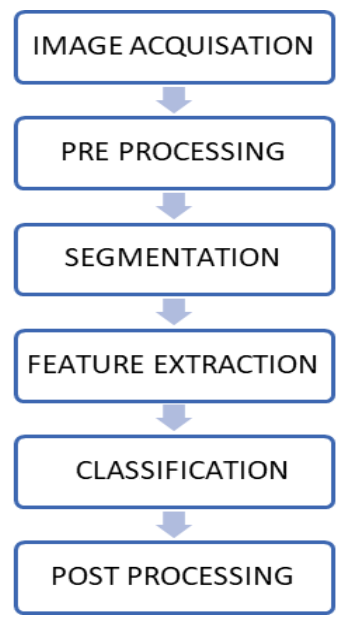
\includegraphics[width=0.3\textwidth]{images/ilustracoes/processo_ocr.png}
\end{wrapfigure}
\noindent
\begin{itemize}
    \item \textbf{Aquisição de input} : imagem a ser reconhecida, incluindo algoritmos de compressão do próprio formato guardado.
    \item  \textbf{Pré processamento} : técnicas de manipulação do input para melhorar resultado de \acrshort{ocr}
    \item \textbf{Segmentação} : segmentação do input, a vários níveis, de modo a isolar o melhor possível os conteúdos relevantes, i.e. o texto.
    \item \textbf{Extração de características} : processo de reconhecimento de características dos caracteres isolados.
    \item \textbf{Classificação} : utilizando as características calculadas é feita a decisão sobre a sua identidade.
    \item \textbf{Pós processamento} : técnicas para melhoria do resultado como, por exemplo, a correção de erros ortográficos. Por vezes pode alterar o documento original se a \gls{ground truth} já contiver estes erros.
\end{itemize}
\noindent

O \textbf{Pré Processamento} é um passo essencial para o aumento do acerto do reconhecimento de texto, sendo que ele pretende remover imperfeições do input como: baixo contraste das linhas, texto mal delimitado, ruído de imagem, orientação do documento ou do texto (principalmente manuscrito). Em alguns casos mais complexos, com ajuda de inteligência artificial, também é possível a reposição de partes parciais de uma imagem que foram perdidas, ou remoção de elementos como \textit{watermarks}.

A \textbf{Segmentação} é usada para isolar o conteúdo útil do resto da imagem podendo envolver vários passos como: segmentação da página para separar texto do resto do conteúdo; segmentação de caracteres, com o intuito de os separar em caracteres individuais, algo que é especialmente difícil com escrita à mão devido à tendência  em criar ligações entre caracteres ou mesmo de os unir; tratamento e normalização dos caracteres isolados - normalização do tamanho, filtração morfológica.

A \textbf{Extração de Características} (Feature Extraction) trata-se do processo de deteção e cálculo das características dos caracteres, para a criação do classificador (dependendo da arquitetura) e anotação do que distingue o caráter alvo. Este processo é possivelmente o mais aberto para variações e que, juntamente com o classificador, mais influencia o resultado. Diferentes técnicas de extração de características e \textbf{Classificação} são utilizadas e foram estudadas durante as últimas décadas: desde \textit{template matching} \citep{10.5555/1074100.1074664} onde são usados algoritmos para cálculo de similaridade entre um template e o alvo, a segmentação de características, como presença de loops ou traços verticais longos  \citep{10.5555/1074100.1074664}, ou distribuições de pixeis \citep{9183326}. 
Para texto humano, este processo torna-se ainda mais complexo devido à necessidade  de lidar com múltiplos caracteres  invés de singulares. 
A classificação passava por um processo de comparação do valor das características calculado com diferentes templates porém, mais recentemente, o uso de estratégias no ramo de machine learning são mais comuns: redes neuronais, support vector machines e k- nearest neighbor; são alguns dos modelos mais utilizados \citep{9183326} \cite{6993174}. Por vezes, o classificador utiliza conhecimento do léxico de uma linguagem para ajudar na sua classificação, sendo que documentos com linguagem desatualizada poderão sofrer nesse caso.

O \textbf{Pós Processamento} é responsável pelo tratamento do output, responsável por mitigar ou corrigir alguns erros do reconhecimento, desde correções ortográficas a posicionamento na página \citep{9183326}.

Este trabalho irá ter como foco principal as secções de pré e pós processamento, e segmentação, na procura de aumentar a eficácia do reconhecimento e da organização dos resultados.



\subsection{Desafios}
\label{ocr_desafios}

\newglossaryentry{ground truth}{
name= ground truth,
description={Em OCR, este é o nome dado ao conteúdo do documento original. Usualmente apenas o conteúdo textual é considerado.}
}

Com a evolução da tecnologia, os problemas foram mudando de foco, tendo passado por um longo período em que a maior prioridade era a capacidade de reconhecimento de caracteres para além de um escopo limitado, tanto em termos de identidade como estilo, para a capacidade de tratar a imagem de forma a que o reconhecimento tenha uma maior taxa de acerto \citep{4283429}.
Alguns dos maiores desafios atualmente para \acrshort{ocr} são:
\begin{itemize}
    \item \textbf{documento original} : danos  no objeto; texto ilegível ou com um tipo de letra muito complexo; linguagem desatualizada; estrutura complexa; inclinação do texto; distorções da página.
    \item \textbf{imagem} : má iluminação; múltiplas páginas com diferentes orientações; baixa resolução; pouco contraste; ruído.
    \item \textbf{classificador ou extrator de features} não adequado para uma dada linguagem.
    \item \textbf{resultado} : validação quando não se tem a \gls{ground truth} disponível
\end{itemize}

Dentro destes, o processamento de estruturas complexas será o foco principal e o expectável maior contributo deste trabalho.


\subsection{Tecnologia}

\newglossaryentry{codec}
{
    name=codec,
    description={Algoritmo de compressão com o propósito de diminuir a dimensão de uma entidade.}
}

\newacronym{ml}{ML}{Machine Learning}

Presentemente, com a proliferação permitida pela internet e a globalização, a disponibilização de ferramentas de \acrshort{ocr}, anteriormente primariamente privilégio de instituições ou empresas, como bancos \citep{10.5555/1074100.1074664}, tornou-se trivial, acessível através de itens do dia a dia como um computador ou telemóvel de forma gratuita, ex.: Google Lens.

Alguns destes softwares que serão utilizados neste trabalho são:
\begin{itemize}
    \item \textbf{Tesseract} 
    \item \textbf{Keras-OCR}
    \item \textbf{PaddleOCR}
\end{itemize}

Os resultados deste tipo software podem ser genericamente descritos como uma lista de caixas, delimitadoras de texto, com conteúdo, i.e. o texto nela contido e, por norma, um nível de confiança no reconhecimento desse texto.

No caso do \textbf{Tesseract} \citep{tesseract_doc}, dentro das várias formas que os resultados podem ser apresentados, a lista de caixas pode ser interpretada como uma árvore de blocos, em que cada nível corresponde a um tipo de estrutura no documento: página $\longrightarrow$ bloco $\longrightarrow$ parágrafo $\longrightarrow$ linha $\longrightarrow$ texto. 

Usando \textbf{PaddleOCR} \citep{paddle_doc}, os resultados são mais simples, divididos apenas pelas linhas de texto detetado.

Já o \textbf{Keras-OCR} \citep{keras_doc} lista um conjunto de caixas em que cada contém uma palavra reconhecida.

Uma outra característica que o \textbf{Tesseract} tem é a capacidade de reconhecer, com nível de acerto variável, outros elementos relevantes de um documento, como imagens ou delimitadores. Isto pode, por outro lado, causar erros na interpretação dos resultados por sobreposição ou multiplicação da quantidade de caixas.  Além disso o \textbf{Tesseract} permite bastantes configurações como: léxico esperado; modo de segmentação; reconhecimento de espaços em branco; etc.

O output deste tipo de software pode ainda ser processado para tomar diversas formas: formatos que apenas retém o conteúdo como texto simples ou markdown;  formatos que mantém informação sobre os blocos detetados, como hOCR.

A validação do output é na maioria dos casos medida a partir da comparação com a \gls{ground truth}, o que limita a capacidade de testar e treinar (no caso de \acrshort{ml} supervisionado) modelos visto que os datasets tem de ser criados de forma minuciosa e consumidora de tempo.

Além dos softwares de reconhecimento, é preciso ter atenção ao tipo dos ficheiros de entrada. Estes são usualmente imagens e, dependendo do tipo de \gls{codec} destes, os algoritmos de compressão aplicados poderão diminuir a qualidade de imagem, como é o caso de formatos \textit{lossy} como \textbf{JPEG}, potencialmente diminuindo o acerto do reconhecimento do texto. \cite{7367194}, no seu estudo demonstra que mesmo entre diferentes tipos de \textit{lossy} \gls{codec} o seu impacto pode variar significativamente nos resultados de \acrshort{ocr}, sendo que o formato \textbf{JPEG}, um dos mais populares, resultou nas menores taxas de sucesso.



\section{Pré Processamento para OCR}
\label{sec_pre_proc_ocr}

\newacronym{dpi}{DPI}{dots per inch}
\newacronym{cnn}{CNN}{Convolutional Neural Network}
\newacronym{gan}{GAN}{Generative Adversarial Network}
\newacronym{psnr}{PSNR}{Peak signal-to-noise ratio}
\newacronym{ssim}{SSIM}{Structural similarity index measure}

Como foi listado na secção \ref{ocr_desafios}, existe uma diversa quantidade de defeitos que os documentos originais e as imagens digitalizadas destes podem ter e cuja presença pode afetar negativamente os resultados de software de \acrshort{ocr}. 
O pré processamento pode ser considerado como uma fase de tratamento de imagem para remover estes problemas que deterioram o reconhecimento de texto. De forma a entender os diferentes métodos utilizados e a sua evolução para o presente, foram selecionados os estudos:  \citep{4283429},\citep{5277501},\citep{9187695},\citep{8545609},\citep{9791698},\citep{8368720},\citep{8269967}.

Entre o grande leque de diferentes algoritmos e tratamentos que podem ser aplicados nas imagens, em geral, estes podem ser segmentados nos mais comuns \citep{9791698}:
\begin{itemize}
    \item \textbf{binarização/thresholding da imagem} : processo de normalização dos pixeis para um de dois valores, mediante um determinado limiar
    \item \textbf{remoção de ruído} : algoritmos para retirar degradações ou sujidades da imagem através de processos como, por exemplo, suavização da imagem calculando para cada pixel o valor médio da sua vizinhança
    \item \textbf{correções de texto} : alguns casos deste são texto que apresenta um ângulo de rotação, texto com inclinação, distorções locais no texto, \textit{watermarks}
    \item \textbf{super-resolução} : aumentar a resolução da imagem, consequentemente aumentando o seu \acrshort{dpi}
    \item \textbf{foco da imagem} : acentuação das arestas, diminuir desfocagem
    \item \textbf{transformações morfológicas} : operações sobre a imagem de modo a provocar maior contraste do conteúdo, ou permitir melhor distinção das características, ex.: dilatação do texto para tornar mais fácil a distinção entre regiões com e sem texto.
\end{itemize}

Para \textbf{binarização}, o objetivo principal é distinguir o texto do resto da imagem, daí a alocação dos pixeis para 1 de dois valores. Este processo é distinguido principalmente entre o uso de \textit{thresholding} global ou local (ou adaptativo), sendo que o global implica um cálculo das características estatísticas locais dentro da imagem, e é mais adequado para o tratamento de imagens com cor, ou com variações de intensidade dispersas pela imagem \citep{9791698}. Alguns dos algoritmos mais comuns são comparados por \cite{9187695}, onde é evidente a dependência destes nas condições do documento original e da imagem. Um exemplo apresentado demonstra como, numa imagem com uma mancha escura (com o texto ainda distinguível), o algoritmo de Otsu conseguiu gerar uma imagem com pouco ruído e bom contraste, mas a zona da mancha fica completamente preta, comparado ao algoritmo de Niblack que, embora com mais ruído, recuperou algum texto dentro da mancha.

A \textbf{remoção de ruído} é possivelmente a área com mais alternativas possíveis e das que mais afeta o resultado do reconhecimento por, a nível de pixeis, o ruído interferir com a composição dos caracteres ou criar acumulações de informação extra que serão mal identificadas pelos softwares, como notado por \cite{4283429}. 
O ruído nas imagens pode ser de vários tipos, o que dificulta a forma de o detetar e tratar. 
Alguns dos outros tratamentos, como a binarização, transformações morfológicas e alguns tipos de super-resolução, também tratam desta questão mesmo não sendo o seu foco principal.  Da mesma forma, alguns dos filtros utilizados podem ter outros resultados como o aumento do contraste ou eliminação de distorções.
Alguns dos tratamentos mais comuns do ruído são\citep{9791698}\citep{8269967}\citep{4283429}:
\begin{itemize}
    \item filtro Gaussiano
    \item médias não locais
    \item suavização com filtro de mínimos locais
    \item suavização com filtro Wiener
\end{itemize}
Vários destes métodos resultam  tanto na acentuação das arestas do texto, como na remoção de lixo ou ruído à sua volta,  recuperando o \textbf{foco da imagem}.

A \textbf{correção de texto} necessita, ao contrário dos outros processos que podem, mesmo sem uma análise prévia do estado da imagem, melhorar o reconhecimento de texto; de uma análise prévia visto que, por exemplo, não se pode aplicar uma rotação na imagem sem saber o ângulo de orientação inicial desta. 
\cite{4283429} faz uma apresentação convincente do efeito de uma rotação de ângulo 15º no reconhecimento do Tesseract, o que impediu o reconhecimento.
O método proposto passa pelo computação de uma linha que afete a margem na extremidade esquerda do texto, de modo a calcular a sua inclinação relativa à margem da imagem e assim descobrir o ângulo de rotação do texto.
No espectro mais limitado da sua proposta, devido à sua localidade nos documentos, \cite{4283429} discute distorções nos documentos como curvaturas resultantes da bainha de um livro. Aqui, em traços gerais, a linha de curvatura do texto é detetada, com a qual é criado um quadrilátero da área afetada, onde será, de acordo com o nível de curvatura na projeção sobre a linha, realizada a correção.
Em ambos os casos, os resultados demonstrados para casos de grande deformação, os algoritmos propostos conseguiram tornar a completa falha de reconhecimento para taxas de acerto dentro dos 99\%.

A aplicação de \textbf{super-resolução} procura auxiliar o processo de reconhecimento ao melhorar a qualidade de imagens de baixa resolução, i.e. aumentar os seus \acrshort{dpi} e tornar os caracteres mais reconhecíveis. 
Entre os vários algoritmos utilizados para este propósito, o uso de interpolação tendia a ser o mais comum, porém nem sempre os resultados eram satisfatórios, resultando em imagens transformadas serem desfocadas, ou com os defeitos originais acentuados, especialmente quando o salto era feito a partir de imagens com \acrshort{dpi} baixo - 100 ou menos \citep{8545609}. No entanto, com os avanços na área das redes neuronais, em particular na categoria de imagens naturais, modelos como \acrshort{cnn} \citep{8368720},\citep{8545609} trouxeram uma nova forma treinar algoritmos para tratar imagens de forma adaptativa e com resultados muito melhores do que os algoritmos bem estabelecidos para este problema. Um dos pontos negativos deste tipo de redes é que a criação de datasets de treino é um processo demorado, sendo que para cada imagem de treino (degradada), é necessário uma imagem par com o resultado ideal para validação do resultado. Adicionalmente estes datasets têm de ter casos com características dispersas o suficiente para permitir uma boa generalização do modelo. Um outro modelo que tem vindo a emergir são as \acrshort{gan} que, invés de utilizarem uma única rede para gerar conteúdo que depois será validado em cada iteração do treino, utilizam duas redes que competem diretamente: a geradora que tenta transformar imagens de modo a enganar o discriminador, e este que tenta entender se a imagem de input é a imagem original ou se foi gerada. \cite{9187695} propõe um modelo deste género que demonstra a sua superioridade tanto em relação a algoritmos baseados em regras, como de modelos baseados em \acrshort{cnn}.

As \textbf{transformações morfológicas} são compostas por vários métodos e propósitos diferentes, nem sempre com o intuito de melhorar a qualidade da imagem, mas para acentuar certas características desta. Por exemplo, técnicas como a dilatação podem ser utilizadas para acentuar regiões de texto de forma a ser possível separar o texto do resto. Por outro lado, técnicas de deteção de arestas, erosão ou \textit{thinning}, diminuem o tamanho dos elementos da imagem, podendo simplificar os caracteres, tornando o seu reconhecimento, ou das suas características (como loops) mais evidentes \citep{9791698}.

Estes diferentes tipos de tratamento podem, na grande maioria dos casos, complementar-se mutuamente e, é costume - inclusive nos estudos referenciados - a criação de pipelines de pré processamento que aplicam estes vários tratamentos de forma sequencial. No entanto, como estes diferentes tratamentos impactam diretamente os dados de input para reconhecimento, nem sempre são benéficos e têm de ser escolhidos com cuidado consoante o estado do sujeito.  \cite{8269967} demonstra precisamente isto mostrando, por exemplo, que a aplicação de um filtro Gaussiano para a redução de ruído num caso de teste reduziu a taxa de acerto do Tesseract para menos de 1 terço comparado ao resultado sem pré processamento. 
Isto naturalmente dificulta a criação de pipelines automáticas de pré processamento. Nesse mesmo estudo, é proposto o uso de uma \acrshort{cnn} que, consoante um número limitado de classes que representam combinações de técnicas de pré processamento, decide a melhor para uma dada imagem. Esta solução resultou numa melhoria considerável, principalmente para o reconhecimento do Tesseract e, mais interessante, a tendência para certas combinações de técnicas com: binarização escolhida \~90\% das vezes, redução de ruído 35\% e acentuação de contrastes 34\%.
Como mencionado anteriormente, os avanços no tratamento de imagem com uso de modelos de Deep Learning vêm trazer, quando suficientemente generalizados, um método ubíquo para a realização destes vários tratamentos de forma adaptativa. \cite{9187695} com a \acrshort{gan} proposta, demonstra resultados no tratamento de ruído, focagem, binarização e remoção de \textit{watermarks} excelentes, mesmo tendo em conta que o foco principal do modelo era o aumento da resolução da imagem original. 

\subsubsection{Métricas de avaliação}
No ato de  pré processamento, as métricas de avaliação são muitas das vezes subjetivas visto, em geral, se tratar de tratamento de imagem e nem sempre haver uma versão não degradada das imagens dos documentos. No caso de haver essa versão prístina, algumas das métricas mais comuns para testar o tratamento de modelos ou algoritmos são: \acrshort{psnr}, que compara o ruído na imagem tratada comparativamente com a original, sendo que valores maiores tendem a significar melhores resultados; e \acrshort{ssim}, que tenta ter em conta as similaridades das vizinhanças na imagem, assim como outros aspetos mais relativos a cor e luminosidade, imagens idênticas terão valor 1. Não havendo a possibilidade de testar com uma imagem base, pode-se avaliar o efeito do pré processamento através da variação dos resultados do output ou do pós processamento.


\section{Pós Processamento para OCR}
\label{sec_pos_proc_ocr}
\newacronym{nlp}{NLP}{Natural Language Processing}
\newacronym{lstm}{LSTM}{Long Short Term Memory}

Na generalidade, o tratamento dos resultados de \acrshort{ocr} ronda em torno das correções sob o texto resultante. Estas correções procuram corrigir erros ortográficos, texto irreconhecível, ou sem sentido (caracteres lixo ou ruído reconhecido).

Correções a nível dos blocos/caixas que englobam o texto reconhecido, são mais orientadas ao tipo de documento e ao seu contexto e serão analisadas com mais atenção nas secções seguintes.

\cite{10.1145/3453476} apresentam um estudo extremamente compreensivo e extenso sobre o estado da arte e o impacto do pós processamento no texto resultante de \acrshort{ocr}.

Neste estudo, é apresentado primeiramente a importância deste tratamento de texto, não só para aumentar a qualidade das aplicações que o utilizam, exemplo dado no caso de \acrshort{nlp}: onde taxas de erro por volta dos 7\% podem mostrar reduções na qualidade da análise de sentimento de até 30\%; mas também no próprio processo de navegação e procura por documentos transcritos por \acrshort{ocr} : em alguns exemplos os erros de texto não permitiram uma indexação ou reconhecimento de termos de pesquisa correta, não sendo devolvidos na procura.

Os dois principais erros de texto reconhecido são:
\begin{itemize}
    \item \textbf{não palavra} : quando uma palavra reconhecida pelo motor de \acrshort{ocr} não se encontra no léxico conhecido
    \item \textbf{palavra real} : a palavra reconhecida pertence ao léxico conhecido, porém difere da \gls{ground truth}
\end{itemize}
Entre estes dois tipos de erro, o primeiro é consideravelmente mais fácil de detetar e potencialmente corrigir, visto o segundo necessitar de informação extra, quer seja esta a \gls{ground truth} do documento - o que é raro -, ou uma análise da palavra dentro do seu contexto.

O estudo segue então para a secção das técnicas de pós processamento. Estas são separadas em dois tipos principais: \textbf{manuais} e \textbf{(semi-)automáticas}.

As técnicas \textbf{manuais} entendem total ação humana e são normalmente dirigidas para projetos mais sensíveis a erros mas que, pela necessidade desta mão de obra, são naturalmente mais custosos, demorados e raros. São casos destes, projetos de transcrição de documentos antigos, como é dado exemplo o projeto da biblioteca nacional da Austrália na correção de jornais históricos.
Alguns outros casos destas técnicas descritos servem mais para o propósito de avaliação de algoritmos ou criação de casos de teste.

As técnicas \textbf{(semi-)automáticas} podem ser agrupadas em dois tipos: \textbf{tratamento de palavras isoladas}, e \textbf{dependentes de contexto}. Dentro destas, o tratamento de palavras isoladas é focado na correção de problemas de 'não palavra', enquanto as dependentes de contexto procuram resolver os dois tipos de problemas.


Dentro das diferentes técnicas baseadas nas \textbf{palavras isoladas}, algumas características servem como fundamentos dos algoritmos:
\begin{itemize}
    \item \textbf{Léxico conhecido}
    \item \textbf{Confiança do reconhecimento}
    \item \textbf{Frequência de utilização de uma palavra, no documento, ou globalmente}
    \item \textbf{Similaridade da palavra errada com as conhecidas no léxico}
\end{itemize}
Entre algumas destas técnicas, são realçadas:

\subsubsection{Junção de Outputs de OCR}

A junção de outputs de OCR visa a escolher entre diferentes resultados para uma dada sequência de palavras, com características distintas (nível de confiança no reconhecimento, quantidade de erros,etc.), e escolher dentro destas ou numa sua mistura, o output final.

Numa 1º fase, os outputs são então obtidos, onde para isto várias propostas foram feitas, com as principais sendo: 
\begin{itemize}
    \item Usando o mesmo motor OCR, fazer vários reconhecimentos de um mesmo trecho de texto
    \item Usando o mesmo motor OCR, fazer vários reconhecimentos de um mesmo trecho de texto, com parâmetros diferentes ou tratamento de imagem diferente
    \item Usando múltiplos motores OCR, fazer vários reconhecimentos de um mesmo trecho de texto
\end{itemize}

Numa 2º fase, estes diferentes outputs têm de ser alinhados de forma a poderem ser comparados palavra a palavra. Para isto, algoritmos sob grafos são comuns.

Por último, utilizando um decisor, o output final é escolhido. Este decisor pode tomar várias formas como: modelos de votação, cálculo de similaridade com léxico, modelos \acrshort{lstm}.

Embora esta técnica geralmente resulte em resultados melhores do que o reconhecimento simples, exige um maior gasto computacional, assim como do facto de estar limitado ao dicionário conhecido.

\subsubsection{Vias lexicais}
Uma outra visão sobre o tratamento do texto, é na procura das palavras mais similares à não palavra detetada e, dentro destas, decidir qual a que tem maior potencial para a substituir. Este cálculo de similaridade pode ser realizado de várias formas, sendo das mais comuns: a distância de Levenshtein, onde se calcula o número de operações mínimas - inserção, remoção ou substituição - a realizar numa palavra para obter outra; variações deste algoritmo; e distância entre n-gramas, que envolve a quantidade de conjuntos de palavras em comum entre as duas palavras comparadas.

Como no caso anterior, estas vias continuam limitadas pelo léxico conhecido, sendo que muito do estudo é dedicado à criação de dicionários mais abrangentes ou adaptados ao documento, ex.: pegando em palavras chaves do documento ou de um tema e criar um dicionário com as páginas mais relevantes de uma pesquisa feita sobre estes.

\subsubsection{Modelos de erro e Máquinas de estado finitas com pesos}
Os modelos de erro procuram calcular as probabilidades sob as operações nos caracteres da palavra errada e, a partir destes e do léxico conhecido, decidir qual o melhor candidato para substituição.

Estes modelos de erro podem ser complementados por máquinas de estados finitas com pesos. Os modelos de erro são utilizados para a escolha de candidatos para substituir o erro, e os pesos da máquina são dependentes de características entre os candidatos e a palavra errada como: comprimento, semelhança, entre outras.

\subsubsection{Modelos de linguagem baseados em tópicos}
No decisão de candidatos para substituição da palavra errada, outros trabalhos sugeriram o uso de contexto do documento de forma parcial, i.e. calcular o tópico do documento a partir da análise deste e utilizar esta informação como um variável extra nas fases de decisão de candidatos. Assim, palavras que sejam numa perspetiva global mais raras não serão tão facilmente descartadas como nos métodos anteriores.

Tal envolve no entanto um processo de decisão sobre quais os tópicos que existem, e a adaptação do léxico para criar correspondências entre as palavras e estes dados tópicos.

\hspace{10pt}

\par Dentro dos métodos \textbf{dependentes de contexto}, são notados os ramos:

\subsubsection{Modelos de linguagem}
\newglossaryentry{word embeddings}
{
name = word embeddings,
description={Forma de vetorização de uma palavra. O vetor de uma palavra representa os seus valores num conjunto de características.}
}

Partindo como base os modelos anteriormente descritos, complementam os modelos com o cálculo da probabilidade de distribuição de sequências de palavras, sendo estas parte do documento. Assim, para cada palavra, utilizando os seus vizinhos, será calculada a probabilidade daquela sequência ocorrer. Este cálculo pode ser calculado utilizando léxicos já definidos, ou complementando estes com as frequências dos n-gramas de palavras dentro do documento. Estes modelos caem dentro do ramo estatístico.

Um outro tipo é conseguido através de redes neuronais que a partir do texto criam \gls{word embeddings}, o que permite calcular a similaridade entre palavras tendo em conta as suas características. Com esta habilidade, as sequências de palavras do texto reconhecido podem ser sujeitas ao cálculo da probabilidade de ocorrerem e, caso este seja muito baixo, poderá ser sinal de um erro de palavra real.

\subsubsection{Machine Learning baseado em características}

Neste caso, o contexto é utilizado dentro de uma quantidade de características mais limitado mas também mais robusto do que na alternativa anterior. Algumas destas características tendem a ser:
\begin{itemize}
    \item Frequência da palavra - nos casos de treino e no próprio documento
    \item Frequência dos ngramas com a palavra -  nos casos de treino e no próprio documento
    \item Peso de confusão - conseguido através dos casos de treino
    \item Confiança do motor OCR na palavra
\end{itemize}

\subsubsection{Seq2Seq - Sequência para Sequência}

Esta alternativa, tem como noção que este problema de correção é uma questão que pode ser resolvida por tradução máquina, correspondendo à transformação numa sequência de palavras, numa outra idêntica ou semelhante, na mesma linguagem.

Estes modelos, ao contrário dos mencionados de modelos de linguagem - que recebendo uma sequência de palavras analisavam a probabilidade de uma outra ser a próxima na sequência, ou sugeriam a próxima palavra -, recebem uma sequência de palavras e devolvem também uma sequência de palavras.

\hspace{10pt}

O estudo termina com uma análise das tendências destas diferentes áreas, onde se pode notar uma aderência maior para tecnologias de inteligência artificial, juntamente com a tendência para a união dos dois ramos de tratamento de texto (semi-)automático nas soluções.


\subsubsection{Métricas de avaliação}
Como acontece no caso do pré processamento, o pós processamento necessita de uma \gls{ground truth} para poder ser avaliado. Contra esta, diferentes medições podem ser feitas, como a percentagem de caracteres ou palavras totais nos dois textos, ou a taxa de acerto tendo em conta alinhamento dos textos. Algumas características como a quantidade de \textit{whitespaces} e indentação também podem ser relevantes para certos tipos de documentos. A quantidade de substituições realizadas, mais propriamente de palavras não reais, também pode ser importante para avaliar o software de reconhecimento, embora este erro possa ser resultado de um léxico não apropriado para o documento, ex.: documentos históricos. 

\section{Segmentação de documentos}
\label{sec_segmentacao_docs}

A segmentação de documentos é um processo que visa decompor o documento nas suas várias secções ou elementos. A sua aplicação pode variar dependendo do objetivo concebido: separação do texto de elementos não texto, retirando informação prejudicial para \acrshort{ocr}; divisão do conteúdo do documento em várias secções para que possam ser analisadas ou extraídas isoladamente. Por este mesmo motivo, estes processo tem aplicabilidade tanto antes como depois de feito o reconhecimento de texto.

\cite{ESKENAZI20171} faz um estudo compreensivo sobre as diferentes metodologias de segmentação de documentos, apresentando as suas diferentes características, evolução e tendências. 
As diferentes técnicas podem ser dividas de forma comum como: 
\begin{itemize}
    \item \textbf{top-down} : divisão a partir da página em blocos mais pequenos
    \item \textbf{bottom-up} : a partir de uma escala mais pequena, ex.: pixeis, componentes conectadas; os elementos são aglomerados em conjuntos maiores até completar a página
    \item \textbf{hibrído}
\end{itemize}

O estudo decide invés seguir por uma divisão em 3 grupos de acordo com a evolução da capacidade dos algoritmos de segmentar diferentes tipos de documentos.
\begin{itemize}
    \item \textbf{Dedicado a um esquema (layout) específico}
    \item \textbf{Capaz de lidar com layouts descritos por um conjunto de parâmetros}
    \item \textbf{Layout potencialmente não restrito}
\end{itemize}

\subsubsection{Algoritmos dedicados a um layout específico}

Estes algoritmos, têm como objetivo a segmentação de um dado tipo de esquema. Estes tendem a ser mais rápidos e, embora os menos versáteis, apresentam para o seu tipo de alvo resultados difíceis de superar. Dentro destes, existem 3 ramos principais de algoritmos. 

O primeiro, são os algoritmos que assumem as características do esquema e, usando estas, criam gramáticas que os descrevem, ou criam perfis do esquema que são projetados nas imagens de input para aplicação de heurísticas de alinhamento e análises probabilísticas para deteção de erros ou desalinhamentos

O segundo ramo, foca-se no uso de filtros para realce de regiões de um layout. Estes são normalmente utilizados para documentos em que as linhas do texto sejam retas e horizontalmente alinhadas. Os casos mais frequentes destes algoritmos aplicam morfologias, como sequências de erosão e dilatação de forma a identificar imagens, ou Run-Length Smoothing para a formação de manchas em áreas densas com conteúdo.

O último ramo, investiga cálculo das linhas que delimitam uma página de forma que uma segmentação em blocos  ocorre naturalmente. Exemplos deste passam pela transformação das linhas do texto em linhas retas; criação de linhas delimitadores através do espaço em branco no documento; transformação de Hough para deteção de linhas.

\subsubsection{Algoritmos que usam parâmetros para descrever um layout}

Estes algoritmos são mais fléxiveis na sua capacidade em lidar com diferentes tipos de documento do que o grupo anterior. Este grupo trabalha com um conjunto de características dos elementos do documento, permitindo assim, com o uso deste contexto extra, mais versatilidade para lidar com irregularidades. Também este grupo pode ser dividido em alguns ramos.

O mais comum destes é o \textit{clustering} onde, partindo de elementos base, como componentes conectadas, procura criar agrupamentos destes, representantes de elementos de ordem superior, como por exemplo imagens, segundo um conjunto de características destes elementos base: geométricas, de textura (distribuição dos pixeis), cor, vizinhança, etc.. Algoritmos híbridos também são usuais, como o uso da informação de uma primeira segmentação em blocos antes de partir para o clustering.

Um outro ramo, trata de fazer o agrupamento de elementos no documento original a partir da otimização de funções de custo. São exemplos destes, algoritmos que iteram sobre a realização de segmentação numa página, onde se estima se a realização de novas segmentações diminui o custo da função.

Por último, e segundo mais popular, estão os algoritmos de classificação. Estes, a partir de um grupo de classes predefinido, pretende atribuir uma delas aos elementos do documento. Este ramo, ao contrário do clustering, é marcado por todos os algoritmos necessitarem de treino. Vários trabalhos deste género, realizam um processo inicial de decisão das melhores features utilizando \acrshort{ml}.

\subsubsection{Algoritmos para segmentação de layout potencialmente não restringidos}

As técnicas mais recentes de segmentação estudadas em \cite{ESKENAZI20171}, englobam um leque de projetos de junção de algoritmos antigos de forma híbrida ou combinada, e algoritmos utilizando redes neuronais. Estes últimos são pouco abordados neste estudo, mas trabalhos recentes, não apenas na segmentação de documentos, mas também em termos de segmentação de imagem, tendem para a utilização de \acrshort{cnn}. Exemplo deste é \cite{8269981}, que usa múltiplas redes convolucionais para a segmentação de uma página entre texto e não texto, e dentro do não texto em figura ou tabela.




\section{Trabalho relacionado}
\label{sec_trab_relacionado}

Nesta secção serão estudados trabalhos cujo objetivo, ou orientação, se assemelha com os objetivos deste projeto, sendo portanto casos de estudo e inspiração relevantes. Os temas abordados são: extração de conteúdo de jornais (\ref{sec_ext_cont_jornais}), e cálculo de ordem de leitura (\ref{sec_ordem_leitura}). Uma última secção é aberta para trabalho futuro que se mostre complementar ao projeto.

\subsection{Extração de conteúdo de jornais}
\label{sec_ext_cont_jornais}

Como argumentado no primeiro capítulo, um dos tipos de documentos que mais sofre no processo de reconhecimento de texto são os jornais. Tal deve-se ao facto de estes terem estruturas complexas, interpoladas com imagens, anúncios, elementos de texto chamativos, porções de texto em contentores irregulares, e outros elementos invulgares que dificultam a criação de heurísticas ou treino de modelos para a sua análise e tratamento.

Nesta secção será feita uma análise de diferentes trabalhos na área de segmentação e extração de conteúdo de jornais. O objetivo da segmentação é geralmente o isolamento dos artigos do jornal.

Estes trabalhos podem ser divididos em dois tipos principais: baseado em \textbf{heurísticas}, ou utilizando \textbf{modelos de machine e deep learning}, maioritariamente \acrshort{cnn}.


\subsubsection{Heurísticas}

\cite{5277572} foi um projeto proposto por elementos da Google que, embora não tão recente como outros, oferece uma visão sobre heurísticas generalizadas para uma grande quantidade de data. Neste trabalho, a parte relevante do processo, i.e. depois da obtenção da imagem do jornal, passa primeiro por um tratamento da imagem, utilizando uma binarização local baseada em morfologias para reconstrução de gradiente cinzento, o que permite a identificação de um contraste entre o conteúdo do documento e o fundo, e consequentemente saturar o fundo. Em seguida, é realizada uma segmentação em blocos através das linhas e "valetas" - trechos do fundo que separam o texto. Depois, é realizada uma análise dos blocos para fazer uma classificação entre títulos e texto considerando o tamanho de fonte e proporção da área do bloco. Os títulos são considerados iniciadores de artigos. Por último, é feita o agrupamento dos blocos em artigos através de duas regras principais: título comum, onde blocos por baixo de um mesmo título fazem parte do mesmo artigo; bloco órfão, onde as exceções à regra anterior são tratadas, juntando blocos órfãos a blocos não órfãos que não tenham blocos por baixo deles e tenham a margem de baixo abaixo da sua margem superior.

O artigo admite acertos de 90\% porém, não suporta estes resultados com números de casos de teste ou identificação de um dataset. Além disso, esta segmentação não tem em conta elementos não texto nos jornais.

\hspace{10pt}

\cite{8300390} apresenta uma outra proposta focado numa primeira segmentação da página utilizando linhas calculadas através de tratamento de imagem, mas elabora no anterior através de uma extensão destas linhas baseado em regras e uma posterior análise da sua distribuição. Ao contrário do trabalho anterior, as imagens são consideradas na segmentação dos artigos e os resultados são apresentados em conjunto com a informação dos testes.

\hspace{10pt}

\cite{6831009} propõe um método híbrido em que são utilizadas heurísticas e grafos para extração do contexto dos blocos, que depois serão classificados usando regressão. Como usual, começam com uma primeira fase de tratamento de imagem para a limpar - binarização, remoção de delimitadores, separar texto de figuras -, e segmentar os blocos em texto e não texto. Numa segunda fase, para cada bloco é calculada a sua vizinhança, sendo que esta é calculada de acordo com um limite de profundidade de adjacência. Para a classificação de blocos e classificação de artigos a profundidade por eles usada é diferente, sendo superior no caso dos artigos. Por fim, os artigos são classificados através de um modelo que tem informação da sua vizinhança, assim como características geométricas do bloco.
Este grafo é denominado de modelo hierárquico de ponto fixo. \cite{8300390} sugerem uma variação deste modelo utilizando um modelo de Markov de 2 dimensões que permite a retenção de possíveis ordens de leitura como contexto adicional.


\subsubsection{Inteligência artificial}

\cite{8999273},\cite{8270006},\cite{Barman_2021} demonstram o poder das \acrshort{cnn} em tarefas de segmentação, sendo capazes de generalizar problemas como linguagens não ocidentais e blocos de conteúdo não retangulares. Esta última habilidade é conseguida através da aplicação de máscaras ao nível dos pixeis invés dos blocos. Além da capacidade de extração de características (visuais) destes modelos, dependendo da sua arquitetura, eles podem ser treinados para realizarem técnicas de tratamento de imagem diretamente \citep{8270006}. \cite{Barman_2021} complementa a arquitetura das \acrshort{cnn} mais genéricas, com a capacidade de analisar características sobre o contexto dos blocos através da modificação da arquitetura para computar \gls{word embeddings} do texto reconhecido.

\hspace{10pt}

Por último, é importante realçar o esforço do projeto Europeana \citep{europeana_pro} na educação e incentivo sobre o processo de digitalização de jornais históricos utilizando \acrshort{ocr}.


\subsection{Ordem de leitura}
\label{sec_ordem_leitura}

No sentido de permitir outras estratégias de extração de conteúdo, passando pela reorganização deste à partida, ou das segmentações resultantes deste, esta secção irá abordar algumas estratégias de cálculo da ordem de leitura.

Na maioria dos documentos, considerando linguagens e estruturas que partilhem as características do português, a ordenação de leitura é relativamente trivial, podendo ser feita uma ordenação topográfica com base em regras geométricas simples como: um bloco está antes dos blocos diretamente por baixo dele; um bloco está antes de blocos à sua direita. Tal não é o caso para documentos que utilizam estruturas mais complexas, ou o contexto do conteúdo como guia da sua ordem de leitura, como jornais, revistas, tabelas, etc.

Este é um problema que está inerentemente ligado ao processo de segmentação de páginas, visto que este último é que provisionará os elementos que depois têm de ser organizados numa ordem de leitura. Dependendo da granulação da segmentação, múltiplos algoritmos de cálculo da ordem de leitura podem ser aplicados para cada nível, como seria o caso de ordenar os diferentes artigos num jornal, e posteriormente ordenar dentro de cada artigo os seus blocos de conteúdo.

\cite{article_ro1} propõe um algoritmo generalista para o cálculo da ordem de leitura de documentos, utilizando um ordenação topológica dos blocos com apenas duas regras: um bloco \textit{a} está antes do bloco \textit{b} se ambos estiverem horizontalmente alinhados (coordenadas x mais à esquerda e mais à direita sobrepõe-se nos dois blocos, tendo em conta uma certa folga) e  \textit{a} está acima de \textit{b}; \textit{a} está antes de \textit{b} se \textit{a} estiver completamente à esquerda de \textit{b}, e não houver nenhum elemento verticalmente entre \textit{a} e \textit{b} que no seu comprimento englobe os dois. Nesta proposta, eles trabalham com blocos ao nível das linhas de texto, porém seria aplicável para blocos de segmentos de texto. Em termos de implementação e lógica, a proposta é bastante simples e competente na generalidade dos casos, porém, como mencionado na introdução da secção, a falta de consideração sobre o contexto impede que certos conflitos entre potenciais ligações de blocos sejam resolvidos da maneira correta.

Bandas desenhadas, tal como jornais, possuem uma estrutura muito variável na sua disposição, mas também na ordem de leitura correta, intendendo por vezes proporcionar experiências ou emoções ao leitor através do modo como o conteúdo é apresentado. São portanto, um bom caso de estudo para o tratamento de jornais. \cite{7351614} implementaram um algoritmo dedicado a este mesmo tipo de entretenimento. A base da solução definida é o uso de grafos e a sua ordenação. Estes são usados para realizar duas ordenações diferentes, uma primeira sob os diferentes painéis de uma página, e um segundo sob as caixas de texto na página. O método de ordenação é simples, sendo novamente geométrico, usando o vizinho mais próximo. Esta simplicidade, é compensada tanto com uma segmentação que é proposta por eles e dedicada a este tipo de documento, e também pela dupla ordenação que, para cada caixa de texto, limita a quantidade de candidatos disponíveis de acordo com a ordem calculada dos painéis.

Numa abordagem não heurística, \cite{9413256} utilizam \acrshort{ml} para ordenação de documentos históricos com estrutura simples e regular, mas que incluem anotações no canto das páginas que alteram a ordem de leitura do texto, tornando-a mais irregular. A proposta passa pelo cálculo da probabilidade entre pares de blocos, que representam a sua hierarquia, por parte de um Multi Layer Percepton. Embora os resultados sejam notáveis na generalidade do dataset proposto, eles notam dificuldades para páginas compostas por tabelas, onde a estrutura é mais complexa. Isto deve-se principalmente ao facto de estas serem uma minoria nos dados de treino. Realça-se aqui a possibilidade de adaptar este, e similares métodos de modelos inteligentes, a partir da criação de datasets dedicados a certos tipos de documentos.



\section{Conclusões}

O estudo realizado para a produção deste capítulo, permitiu uma clarificação das bases relativas ao trabalho com motores de \acrshort{ocr}, as boas práticas e procedimentos comuns no seu tratamento e melhoria, e os efeitos que, em especial, pré processamento de imagens e pós processamento de texto podem ter sob o resultado final. Além disso, na secção \ref{sec_trab_relacionado}, o estudo de trabalhos com temática similar ou sobre técnicas relevantes para o projeto atual, permitiu uma melhor perceção sobre os fluxos da solução destes e, simultaneamente, entender os maiores desafios com que se deparam - solucionados e por solucionar. Além disso, realça-se que tal como em várias outras áreas tecnológicas, tem nos últimos anos havido uma imergência de soluções com recurso a Inteligência Artificial, com principal sucesso no ramo de tratamento de imagem.

O acumular deste estudo permitiu então um desenho da solução final e do plano de tarefas mais coerente e fundado nos produtos e evolução da área em que se insere, i.e. reconhecimento óptico de caracteres para extração de conhecimento.


\chapter{O problema e os seus desafios}
\label{cap_problema}


Neste capítulo, é feita uma síntese dos desafios do problema e uma discussão sobre a solução desenhada até ao momento para concretizar os objetivos definidos.

\section{Desafios}

No capítulo \ref{cap_estado_arte}, realizou-se um estudo abrangente sobre o estado da arte no que toca a projetos que utilizem \acrshort{ocr} e trabalhos relacionados com os objetivos listados para este projeto (\ref{section_objetivos}).  Através deste estudo, foi possível extrair um leque de problemas detetados na utilização de reconhecimento de texto em documentos, de forma generalizada ou para tipos específicos como é o caso deste trabalho. Em suma, os principais desafios são:
\begin{itemize}
    \item \textbf{Problemas de imagem} : tanto na imagem de input, como no documento original. Ex.: ruído, baixa resolução, má iluminação.
    \item \textbf{Problemas de reconhecimento} : estes são muitas vezes derivados do conjunto anterior, mas outras questões como léxico no documento desconhecido pelo motor OCR ou estruturas complexas podem provocar erros no reconhecimento.
    \item \textbf{Problemas nos resultados} : consideremos estes os problemas sobre as entidades reconhecidas pelo software, tanto o texto que em muitos casos apresenta erros como os próprios contentores em que estes são incluídos.
    \item \textbf{Problemas na extração de conteúdo} : no processo de criação de output, por vezes questões como a ordem de leitura dos blocos identificados, ou reposição de elementos não texto têm de ser abordados.
    \item \textbf{Validação da implementação} : de forma a verificar a eficácia da solução criada, geralmente datasets de teste e casos de estudo relevantes têm de ser criados.
\end{itemize}


\section{Plano da Solução}
\begin{wrapfigure}{r}{0.3\textwidth}
    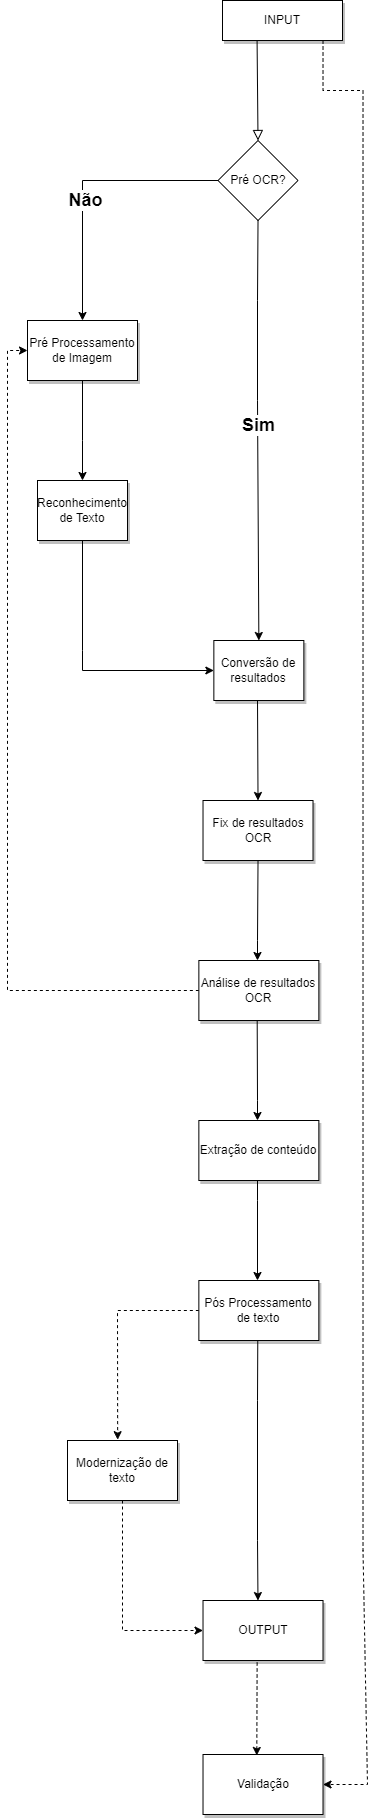
\includegraphics[width=0.25\textwidth]{images//diagramas/pipeline_geral.png}
    \caption{Pipeline da solução}
    \label{fig:pipeline_geral}
\end{wrapfigure}
Durante o estudo do estado da arte, tornou-se evidente que a maioria dos trabalhos com vista em extrair ou corrigir a extração de documentos utilizando reconhecimento de texto, de forma a manter o conteúdo e lógica original, seguem uma metodologia semelhante: uma primeira fase de pré processamento da imagem de input; possível segmentação da imagem entre texto e não texto; reconhecimento de texto; pós processamento do texto; possível pós processamento para segmentação de conteúdo específico de um tipo de ficheiro, como artigos, ou para reorganização dos resultados (ordem de leitura); criação de output.

Partindo desta base, a figura \ref{fig:pipeline_geral} representa o fluxo da solução planeada atualmente. 

A pipeline começa com a introdução de um input, podendo este ser sujeito de reconhecimento de texto, no caso de ser uma imagem, ou já possuir os resultados de reconhecimento, como hOCR. No caso de uma imagem, antes de ser aplicado o software de OCR, será realizado pré processamento da imagem para aumentar a chance de bons resultados de OCR.

Os resultados de OCR são então convertidos para uma estrutura de dados genérica, de modo a englobar os diferentes tipos de resultados possíveis de diferentes tipos de ficheiros ou motores de OCR. Em diante, esta estrutura será usada nos módulos que utilizam os resultados de OCR.

Depois, passa-se por um processo de pós processamento básico dos resultados de OCR. Tal tem o intuito de corrigir erros menos severos no que toca às \textit{bounding boxes} dos resultados e lixo reconhecido pelo motor.

Uma análise dos resultados limpos é então realizada, extraindo informação sobre o texto reconhecido, estimas do possível layout, erros de reconhecimento, etc.. Com os resultados da análise feita, abre-se a possibilidade de realizar um tratamento de imagem diferente dedicado à resolução de problemas detetados, por exemplo: detetado um \acrshort{dpi} de imagem muito baixo, este é um indicador de que a resolução da imagem poderia ser aumentado para melhorar o reconhecimento, procedimento comum no estudo feito.

Utilizando os resultados da análise, são de pois aplicados algoritmos para extração do conteúdo do documento. Aqui o principal objetivo será o cálculo da ordem de leitura e agrupamento dos elementos em conjuntos como artigos.
Além disso, o objetivo secundário envolvente da modernização de texto poderá nesta etapa ser aplicado.

Finalmente, o output final é gerado. Diferentes formas de output serão disponibilizadas dependendo da estrutura pretendida, por exemplo: markdown ou texto simples no caso de apenas se querer os elementos do texto isolado; html para reconstruir a estrutura do documento original. 



\part{\textit{Core} da Dissertação}

\chapter{Contribuição}
\label{cap_contribuicao}

Nesta secção, será relatado o trabalho realizado no intuito da componente prática do projeto e os resultados. 
% Neste caso, relevante à criação de um \textit{toolkit} e ferramentas para a extração do conteúdo de documentos antigos, em particular jornais, com melhores resultados do que os oferecidos pelas ferramentas de \acrshort{ocr} base e, possibilitando a obtenção da lógica e organização original dos mesmos.

\section{Introdução}
% Ao longo do período de inicialização da dissertação: desde a definição dos objetivos do projeto, aprofundamento da temática e estudo do estado da arte; de forma a simultaneamente acostumar com as tecnologias, assim como ganhar um melhor entendimento sobre os algoritmos a implementar e os desafios apresentados, algum trabalho prático já foi realizado. 
% Este envolve principalmente a criação de uma ferramenta para facilitar a visualização dos resultados de reconhecimento, assim como o debugging destes e alguns algoritmos preliminares para manipulação destes resultados de \acrshort{ocr}.

A discussão sobre o trabalho realizado será estruturada em 3 componentes principais.
\begin{itemize}
	\item Ferramentas do \textit{toolkit} desenvolvidas \ref{contribution_toolkit}
	\item Pipeline de aplicação do toolkit \ref{contribution_toolkit_pipeline}
% 	\item GUI de aplicação geral do \textit{toolkit}
	\item GUI editor OCR \ref{contribution_ocr_editor}
\end{itemize}

Para cada uma das secções delimitadas, será dada uma explicação do seu propósito e produto sumariado, procedido por uma discussão mais detalhada dos elementos que a constituem.

De forma geral, o código desenvolvido foi maioritariamente escrito em Python, com algumas instâncias de C.

\section{Ferramentas do \textit{toolkit} desenvolvidas}
\label{contribution_toolkit}

\subsection{Introdução}

A componente do \textit{toolkit} foi a premissa base do tema da dissertação. Um conjunto de ferramentas focado na melhoria dos resultados obtidos da aplicação de \acrshort{ocr} em documentos antigos, com especial interesse em jornais. 

Estas ferramentas são então pertinentes para os diversos passos do processo convencional de \acrshort{ocr}, i.e. pré-processamento, OCR e pós-processamento; atendendo tanto a processamento de imagem, processamento de resultados de OCR e texto, e validação de resultados.

Além dos métodos principais criados para a resolução de problemas identificados, é importante realçar certos pontos essenciais que serviram como base para o resto do trabalho. Estes são as estruturas de dados utilizadas para o tratamento dos resultados de OCR.

\subsection{Sumário}

\begin{itemize}\setlength\itemsep{-0.3em}
	\item Estruturas de dados \ref{data_structures}
	\begin{itemize}\setlength\itemsep{-0.3em}
		\item OCR Tree \ref{ocr_tree}
		\item Box \ref{box_data_structure}
	\end{itemize}
	\item Métodos \ref{contribution_methods}
	
	\begin{itemize}\setlength\itemsep{-0.3em}
		\item Processamento de resultados OCR \ref{contribution_ocr_posprocessing}
		
		\begin{itemize}\setlength\itemsep{-0.3em}
			\item Conversão de resultados OCR \ref{ocr_results_conversion}
			\item Debugging \ref{contribution_debugging}
			\item Análise de texto \ref{contribution_text_analyses}
			\item Limpeza de OCR Tree \ref{contribution_clean_ocr}
			\item Categorização de Blocos \ref{contribution_categorize_blocks}
			\item Divisão de blocos \ref{contribution_divide_blocks}
			\item Cálculo de ordem de leitura \ref{contribution_reading_order}
			\item Segmentação de resultados \ref{contribution_result_segmentation}
		\end{itemize}
		
		\item Processamento de imagem \ref{contribution_image_processing}
		\begin{itemize}\setlength\itemsep{-0.3em}
			\item Binarização de imagem
			\item Rotação de imagem
			\item Cálculo de sentido de rotação
			\item Segmentação de documento
			\item Identificação de imagens
			\item Identificação de delimitadores
			\item Divisão de colunas 
		\end{itemize}
		
		\item Processamento de texto \ref{contribution_text_processing}
		\begin{itemize}\setlength\itemsep{-0.3em}
			\item Limpeza de hifenização
		\end{itemize}
		
	
	
		\item Validação de resultados \ref{contribution_results_validation}
	\end{itemize}
\end{itemize}


\subsection{Estruturas de dados}
\label{data_structures}


\subsubsection{OCR Tree}
\label{ocr_tree}

Como o produto final do projeto intende aceitar diferentes tipos de resultados OCR, i.e. resultantes de diferentes motores OCR ou de ficheiros como hOCR que já possuem os resultados, existe uma necessidade de converter estes diferentes formatos num único tipo que mantenha a informação base pretendida.

Estruturas de dados standard como \citep{hocr_doc} ou \citep{alto_doc} apresentam um resultado final semelhante e com capacidade base de armazenamento de meta-dados superior porém, sendo baseados em XML, tornam a sua manipulação mais complexa e, em múltiplos casos a informação proporcionada é além do necessário ou gera conclusões erradas quando gerado de output automático (ex.: atribuição de classes caption a blocos que são títulos). Assim sendo, embora tenha sido desenvolvido um conversor de, e para HOCR, para o atual projeto, optou-se pela criação de uma estrutura de dados própria.

Deste modo, tomando como inspiração os atributos dos resultados do Tesseract no modo de dicionário \citep{tesseract_doc}, foi implementada uma estrutura de dados no formato de árvore de dados.

A escolha de uma estrutura de árvore permite a hierarquização de blocos de acordo com o seu nível, quer exista uma divisão de nível à partida, como é o caso do Tesseract que segue: página $\longrightarrow$ bloco $\longrightarrow$ parágrafo $\longrightarrow$ linha $\longrightarrow$ palavra; ou apenas um único nível, semelhante ao Keras-OCR.

Todos os algoritmos desenvolvidos, inclusive os métodos para visualização (métodos de debugging e GUI desenvolvido), assumem e trabalham com os dados de OCR no formato desta estrutura de dados.

As características mais relevantes desta estrutura são:

\begin{itemize}\setlength\itemsep{-0.3em}
	\item \textbf{Level} : Nível/altura do nodo.
	\begin{itemize}\setlength\itemsep{-0.3em}
		\item documento : 0
		\item página 	: 1
		\item bloco		: 2
		\item parágrafo : 3
		\item linha 	: 4
		\item palavra	: 5
	\end{itemize}\setlength\itemsep{-0.3em}
	\item \textbf{(page|block|par|line|word)\_num}: Identificação da ordem (dentro de outras caixas(ex.: linha), se aplicável)
	\item \textbf{text} : Texto do bloco, normalmente apenas preenchido ao nível da palavra
	\item \textbf{conf} : Confiança no texto
	\item \textbf{id}
	\item \textbf{type} : Tipo do bloco, ex.: delimitador, título
	\item \textbf{children}
	\item \textbf{box}: Bounding box do nodo, representado pela estrutura de dados Box, que também possui métodos para transformações e verificações geométricas ou de características.
	\item Características de texto: ex.: texto iniciado (start\_text); texto não terminado (end\_text).
\end{itemize}

%% TODO : Ilustracao de uso de arvore OCR para demonstrar diferentes niveis de um documento

Construtores da classe são capazes de admitir outros atributos não base de modo a expandir a utilidade da estrutura. Construtores disponíveis: iniciação por argumentos, dicionário, ficheiro JSON e ficheiro HOCR.

Da mesma forma, conversores para estes ficheiros compreendidos para iniciação também foram desenvolvidos.

A classe possuí por métodos de transformação e análise sobre a árvore OCR que facilitam a manipulação dos resultados OCR. 

Segue-se uma lista dos métodos mais relevantes disponíveis da classe.

\highlight{id\_boxes}
 
 
\textbf{Descrição:} Adiciona identificador aos blocos.
	
\textbf{Argumentos:}
	\begin{itemize}\setlength\itemsep{-0.3em}
		\item level : lista de níveis onde adicionar identificador
		\item ids (opt): dicionário de ids a utilizar caso não se queira iniciar no 0.
		\item delimiters (opt): flag para identificar delimitadores
		\item area (opt): argumento do tipo Box, que restringe os nodos a identificar a uma dada área
		\item override (opt): flag para reescrever id se já existe.
	\end{itemize}
				
\highlight{calculate\_mean\_height}

\textbf{Descrição:} Calcula a altura média das caixas de um dado nível.
	
\textbf{Argumentos:}
\begin{itemize}\setlength\itemsep{-0.3em}
	\item level : nível a calcular
	\item conf (opt): valor de confiança de texto no caso de apenas serem relevantes caixas com certa confiança (aplicável apenas para nível de texto)
\end{itemize}

	
\highlight{is\_text\_size}

\textbf{Descrição:} Verifica se um nodo se encontra dentro do tamanho de texto.
	
\textbf{Argumentos:}
\begin{itemize}\setlength\itemsep{-0.3em}
	\item text\_size : tamanho de texto a comparar
	\item mean\_height (opt): altura do bloco, caso já tenha sido calculado
	\item range : margem de erro aceitável (relativo)
	\item level : nível das caixas usado caso seja necessário calcular a altura média
	\item conf : confiança do texto a utilizar para calcular a altura média
\end{itemize}

\highlight{is\_empty}

\textbf{Descrição:} Verifica se um nodo é vazio.
	
\textbf{Argumentos:}
\begin{itemize}\setlength\itemsep{-0.3em}
	\item conf : confiança de texto a utilizar para considerar palavras válidas
	\item only\_text : flag que dita se o tipo do bloco influencia o resultado, i.e. blocos de tipo "image" não são vazios
\end{itemize}

	
\highlight{text\_is\_title}

\textbf{Descrição:} Verifica se um nodo é potencial título.
	
\textbf{Algoritmo:} Caixa não é texto vertical e é maior do que o tamanho normal de texto.


\textbf{Argumentos:}
\begin{itemize}\setlength\itemsep{-0.3em}
	\item normal\_text\_size : tamanho de texto considerado como normal
	\item conf : confiança de texto a utilizar para considerar palavras válidas
	\item range : margem de acerto aceitável (relativo)
	\item level : nível usado para calcular o tamanho médio do bloco
\end{itemize}

	
\highlight{is\_delimiter}

\textbf{Descrição:} Verifica se um nodo é potencial delimitador.
	
\textbf{Algoritmo:} Caixa já é do tipo delimitador, ou é vazia e segue a regra:

$ box.width >= box.height*4 || box.height >= box.widht*4 $.


\textbf{Argumentos:}
\begin{itemize}\setlength\itemsep{-0.3em}
	\item conf : confiança de texto a utilizar para considerar palavras válidas
	\item only\_type : flag que dita se usa apenas o tipo do nodo para a verificação
\end{itemize}

	
\highlight{is\_image}

\textbf{Descrição:} Verifica se um nodo é potencial imagem.
	
\textbf{Algoritmo:} Caixa já é do tipo imagem ou, é vazia, não é um delimitador e é 3 vezes mais alta do que o tamanho de texto.


\textbf{Argumentos:}
\begin{itemize}\setlength\itemsep{-0.3em}
	\item conf : confiança de texto a utilizar para considerar palavras válidas
	\item text\_size : tamanho de texto a utilizar para comparação com altura da caixa
	\item only\_type : flag que dita se usa apenas o tipo do nodo para a verificação
\end{itemize}


\highlight{get\_boxes\_in\_area}

\textbf{Descrição:} Obtém todas as caixas numa dada área.


\textbf{Argumentos:}
\begin{itemize}\setlength\itemsep{-0.3em}
	\item area : área de interesse
	\item level : nível dos nodos a ir buscas. Se nível == -1, obtém todos os nodos
	\item conf : confiança de texto a utilizar para considerar nodos válidos
	\item ignore\_type : tipos de nodo a ignorar
\end{itemize}
	
	
\highlight{is\_vertical\_text}

\textbf{Descrição:} Verifica se um nodo é texto vertical.

\textbf{Argumentos:}
\begin{itemize}\setlength\itemsep{-0.3em}
	\item conf : confiança de texto a utilizar para considerar palavras válidas
\end{itemize}
	
\textbf{Algoritmo:}

\begin{breakablealgorithm}
	\caption{Verificação de texto vertical}
	\footnotesize
	\begin{algorithmic}[1]
		\If{nodo não é vazio}
			\State lines
			\If{len(lines) == 0}
				\Return False
			\EndIf
			\State \textit{// Linha única}
			\If{len(lines) == 1}
				\State words
			 \State \textit{// Palavra única}
				\If{len(words) == 1}
					\If{altura da palavra >= 2 * largura da palavra}
						\Return True
					\EndIf
				\State \textit{// Múltiplas palavras} 
				
				\Else
					\State \textit{// Verifica se a maioria das palavras coincidem horizontalmente}
					\State widest\_word <- calcula palavra mais larga
					\State overlapped\_words = 0
					\For{word in words}
						\If{word == widest\_word}
							\State continue
						\EndIf
						\If{word.box.within\_horizontal\_boxes(widest\_word.box,range=0.1)}
							\State overlapped\_words += 1
						\EndIf
					\EndFor
					\If{overlapped\_words/len(words) >= 0.5}
						\Return True
					\EndIf
					
				\EndIf
				
			\State \textit{// Múltiplas linhas} 
			
			\Else
				\State \textit{// Verifica se a maioria das linhas coincidem verticalmente}
				\State tallest\_line <- calcula linha mais alta
				\State overlapped\_lines = 0
				
				\For{line in lines}
					\If{line == tallest\_line}
						\State continue
					\EndIf
					\If{line.box.withinvertical\_boxes(tallest\_line.box,range=0.1)}
						\State overlapped\_lines += 1
					\EndIf
				\EndFor
				\If{overlapped\_lines/len(lines) >= 0.5}
					\Return True
				\EndIf
			
			\EndIf
			
		\EndIf
		
		\Return	False
		
	\end{algorithmic}
\end{breakablealgorithm}



\highlight{prune\_children\_area}

\textbf{Descrição:} Atualiza dimensões dos filhos de um nodo para se encaixarem dentro de uma área.


\textbf{Argumentos:}
\begin{itemize}\setlength\itemsep{-0.3em}
	\item area : área de interesse
\end{itemize}


\highlight{boxes\_below}
(método semelhante para as outras direções)

\textbf{Descrição:} Dada uma lista de OCR Tree, devolve aqueles que se encontram por baixo do bloco atual. Os blocos filtrados podem intersetar ou estar dentro do bloco comparado.


\textbf{Argumentos:}
\begin{itemize}\setlength\itemsep{-0.3em}
	\item blocks : lista de blocos a filtrar
\end{itemize}



\highlight{boxes\_directly\_below}
(método semelhante para as outras direções)

\textbf{Descrição:} Dada uma lista de OCR Tree, devolve aqueles que se encontram diretamente por baixo do bloco atual. Blocos filtrados não estão dentro do bloco comparado e não podem estar diretamente por baixo dos outros blocos.


\textbf{Argumentos:}
\begin{itemize}\setlength\itemsep{-0.3em}
	\item blocks : lista de blocos a filtrar
\end{itemize}
	
	
	
\highlight{join\_trees}

\textbf{Descrição:} Junta duas OCR Tree com do mesmo nível numa única árvore. Tem dois métodos principais de junção das árvores: vertical, operação mais simples em que basicamente apenas se juntam as duas listas de ramos dos nodos raíz (assume-se que uma das árvores é mais alta do que a outra e não se intersetam); e horizontal, onde se procura juntar árvores que têm interseção no eixo y, sendo necessário verificar as posições que os filhos devem tomar e se certos filhos devem ser unidos num único (podendo resultar numa junção de linhas).

%% TODO : ilustração poderá ajudar


\textbf{Argumentos:}
\begin{itemize}\setlength\itemsep{-0.3em}
	\item tree : árvore a juntar
	\item orientation : orientação da junção, vertical ou horizontal.
\end{itemize}

\textbf{Algoritmo:}

\begin{breakablealgorithm}
	\caption{Junção horizontal}
	\footnotesize
	\begin{algorithmic}[1]
		\State tree\_children
		\State self\_children
		\State \textit{// no último nível, filhos são ordenados da esquerda para a direita}
		\If{último nível da tree}
			\State tree\_children $\leftarrow$ ordenar lista da esquerda para a direita
		\EndIf
		
		\For{child in tree\_children}
			\If{não é o último nível}
				\State self\_children $\leftarrow$ ordena de cima para baixo
				\If{child pode ser inserida no topo ou fundo da lista}
					\State self\_children $\leftarrow$ insere child no início ou fim
				\Else
					\State \textit{// procura slot para inserir, ou nodo com quem unir}
					\State joined = False
					\For{i in range(len(self\_children))}
						\If{child não interseta com nodo i ou nodo i+1}
							\State self.children $\leftarrow$ adiciona child entre os dois nodos
							\State joined = True
						\\ElsIf{interseta com nodo i}
							\If{interseção em pelo menos 70\% da altura da caixa}
								\If{nodo i tem filhos}
									\State \textit{// join recursivo}
									\State self\_children[i].join\_trees(child,orientation=orientation)
								\Else
									\State self\_children $\leftarrow$ insere child depois do nodo i
								\EndIf
								\State joined = True
							\Else
								\State \textit{// procura local mais baixo para inserir (por poder intersetar com varios blocos)}
								\For{j in range(i,len(self\_children))}
									\If{nodo j mais alto do que child}
										\State self\_children $\leftarrow$ insere child depois do nodo j
										\State joined = True
									\EndIf
								\EndFor
								\If{not joined}
									\State self\_children $\leftarrow$ insere child no fim
									\State joined = True
								\EndIf
							\EndIf
						\EndIf
						
						\If{joined}
							\State break
						\EndIf
					\EndFor
				\EndIf
			\Else
				\State self.children $\leftarrow$ adiciona child no fim da lista
			\EndIf
			
			\State self\_children $\leftarrow$ atualiza lista de filhos
		\EndFor
		
		
	\end{algorithmic}
\end{breakablealgorithm}


\highlight{remove\_blocks\_inside}

\textbf{Descrição:} Remove os blocos dentro do bloco com dado id. Blocos removidos são do mesmo nível que o bloco com dado id.


\textbf{Argumentos:}
\begin{itemize}\setlength\itemsep{-0.3em}
	\item id : id do bloco a limpar
	\item block\_level : nível do bloco a limpar
\end{itemize}

\highlight{update\_position}

\textbf{Descrição:} Atualiza a posição da bounding box de um nodo e dos seus filhos. Especialmente útil para o editor OCR.


\textbf{Argumentos:}
\begin{itemize}\setlength\itemsep{-0.3em}
	\item top : valor a atualizar verticalmente
	\item left : valor a atualizar horizontalmente
	\item absolute : flag que indica se operação é de do tipo absoluta, i.e. bounding box vai ser diretamente atualizada com estes valores, ou relativa, aos valores da bounding box serão somados os argumentos
\end{itemize}

\highlight{update\_size}

\textbf{Descrição:} Atualiza o tamanho da bounding box de um nodo e dos seus filhos nas arestas (filhos interiores não serão alterados). Especialmente útil para o editor OCR.


\textbf{Argumentos:}
\begin{itemize}\setlength\itemsep{-0.3em}
	\item top : valor a atualizar ao topo
	\item left : valor a atualizar à esquerda
	\item bottom : valor a atualizar ao fundo
	\item right : valor a atualizar à direita
	\item absolute : flag que indica se operação é de do tipo absoluta, i.e. bounding box vai ser diretamente atualizada com estes valores, ou relativa, aos valores da bounding box serão somados os argumentos
\end{itemize}

\highlight{update\_box}

\textbf{Descrição:} Atualiza diretamente valor da bounding box do nodo e dos filhos. Especialmente útil para o editor OCR.

\textbf{Argumentos:}
\begin{itemize}\setlength\itemsep{-0.3em}
	\item top : valor a atualizar ao topo
	\item left : valor a atualizar à esquerda
	\item bottom : valor a atualizar ao fundo
	\item right : valor a atualizar à direita
	\item children : flag que indica se é para se aplicar ajuste direto no nodo, ou apenas ajustar de forma a não sair da bounding box do pai.
\end{itemize}

\highlight{scale\_dimensions}

\textbf{Descrição:} Escala dimensões da bounding box do nodo e dos seus filhos. Especialmente útil para o editor OCR.

\textbf{Argumentos:}
\begin{itemize}\setlength\itemsep{-0.3em}
	\item scale\_width : escalar de valores do eixo horizontal
	\item scale\_height : escalar de valores do eixo vertical
\end{itemize}


\subsubsection{Box}
\label{box_data_structure}

A estrutura de dados Box é utilizada maioritariamente para encapsular os dados das bounding boxes dos resultados de OCR. Embora em geral este tipo de dados seja geralmente fornecido por métodos de módulos de manipulação de imagens na forma de tuplo, a utilização de uma classe dedicada permite o desenvolvimento e utilização de métodos para sua manipulação de forma mais simples e organizada.

Tal como a estrutura de dados OCR Tree, esta classe apresenta construtores e conversores de ficheiros diferentes tipos: argumentos simples, dicionário, ficheiro JSON.

Os principais atributos da estrutura são:

\begin{itemize}\setlength\itemsep{-0.3em}
	\item \textbf{left} 	: Valor mais à esquerda da caixa.
	\item \textbf{right}	: Valor mais à direita da caixa.
	\item \textbf{top} 		: Valor mais em cima da caixa (menor do que bottom por ser baseado em manipulação de imagem). 
	\item \textbf{bottom} 	: Valor mais em baixo da caixa.
	\item \textbf{width} 	: Comprimento da caixa.
	\item \textbf{height} 	: Altura da caixa.
\end{itemize}

Realça-se que os atributos desta classe são esperados no formato de inteiros, devido a ter como foco o seu uso no contexto do espaço de imagens.

Segue-se uma lista dos métodos mais relevantes disponíveis da classe.

\highlight{update}

\textbf{Descrição:} Atualiza os valores dos atributos de posição da caixa. Atributos de posição são mantidos válidos, i.e. left <= right e top <= bottom . Altura e comprimento são atualizados automaticamente.

\textbf{Argumentos:}
\begin{itemize}\setlength\itemsep{-0.3em}
	\item top : valor a atualizar ao topo
	\item left : valor a atualizar à esquerda
	\item bottom : valor a atualizar ao fundo
	\item right : valor a atualizar à direita
\end{itemize}


\highlight{move}

\textbf{Descrição:} Soma valores aos atributos de posição da caixa.

\textbf{Argumentos:}
\begin{itemize}\setlength\itemsep{-0.3em}
	\item x : valor a somar nos atributos de posição horizontais
	\item y : valor a somar nos atributos de posição verticais
\end{itemize}

\highlight{within\_vertical\_boxes}
(método semelhante para direção horizontal)

\textbf{Descrição:} Verifica se caixa e caixa a ser comparada estão alinhadas verticalmente, podendo considerar uma margem de acerto. Verificação é realizada nos dois sentidos, i.e. caixa 1 alinhada com caixa 2 ou vice-versa.

\textbf{Argumentos:}
\begin{itemize}\setlength\itemsep{-0.3em}
	\item box : caixa a comparar
	\item range : valor relativo da altura da caixa, a servir como margem para considerar na verificação
\end{itemize}

\highlight{is\_inside\_box}

\textbf{Descrição:} Verifica se caixa a ser comparada está dentro da caixa. Caixa a ser compara tem de estar completamente dentro para resultado afirmativo.

\textbf{Argumentos:}
\begin{itemize}\setlength\itemsep{-0.3em}
	\item box : caixa a comparar
\end{itemize}


\highlight{intersects\_box}

\textbf{Descrição:} Verifica se caixa a ser comparada interseta com a caixa.

\textbf{Argumentos:}
\begin{itemize}\setlength\itemsep{-0.3em}
	\item box : caixa a comparar
	\item extend\_vertical : flag para indicar se verificação deve ser feita apenas longo do eixo x (ex.: utilizado para verificar se caixa comparada está diretamente por acima da caixa)
	\item extend\_horizontal : flag para indicar se verificação deve ser feita apenas longo do eixo y (ex.: utilizado para verificar se caixa comparada está diretamente à direita caixa)
	\item inside : flag para indicar se verificação de caixa dentro conta como interseção
\end{itemize}


\highlight{intersect\_area\_box}

\textbf{Descrição:} Calcula a caixa de interseção entre a caixa e uma caixa a comparar.

\textbf{Argumentos:}
\begin{itemize}\setlength\itemsep{-0.3em}
	\item box : caixa a comparar
\end{itemize}


\highlight{remove\_box\_area}

\textbf{Descrição:} Remove área da caixa. Procura remover área aplicando as menores modificações possíveis. Apenas realiza modificações, se área fornecida está dentro da caixa.

\textbf{Argumentos:}
\begin{itemize}\setlength\itemsep{-0.3em}
	\item area : area da caixa a remover
\end{itemize}


\highlight{get\_box\_orientation}

\textbf{Descrição:} Método naive para obter orientação da caixa (horizontal, vertical ou square) de acordo com a diferença entre a sua altura e comprimento.


\highlight{join}

\textbf{Descrição:} Une duas caixas.

\textbf{Argumentos:}
\begin{itemize}\setlength\itemsep{-0.3em}
	\item box : caixa a unir
\end{itemize}

\highlight{distance\_to}

\textbf{Descrição:} Calcula distância entre duas caixas. Procura dois pontos mais próximos de acordo com argumentos dados e utiliza distância euclidiana para calcular a distância.

\textbf{Argumentos:}
\begin{itemize}\setlength\itemsep{-0.3em}
	\item box : caixa a comparar
	\item border (opt): borda da caixa a ter em conta. Valores disponíveis: "left", "right", "top", "bottom", "closest". Se "closest" for fornecido, procura a menor distância entre bordas. Se nenhum valor for fornecido, utilizado os pontos centrais das caixas.
\end{itemize}


\highlight{distance\_to\_point}

\textbf{Descrição:} Calcula distância entre a caixa e um ponto. Procura calcular a menor distância da caixa ao ponto (tendo em conta a diferença entre o ponto e as bordas).

\textbf{Argumentos:}
\begin{itemize}\setlength\itemsep{-0.3em}
	\item x : valor x do ponto
	\item y : valor y do ponto
\end{itemize}

\highlight{vertices}

\textbf{Descrição:} Retorna uma lista dos vértices da caixa na forma de tuplos (x,y) seguindo de cima para baixo, esquerda para a direita.


\highlight{closest\_edge\_point}

\textbf{Descrição:} Calcula a borda mais próxima entre a caixa e um ponto. Utilizado no editor de resultados OCR para operações de divisão de blocos.

\textbf{Argumentos:}
\begin{itemize}\setlength\itemsep{-0.3em}
	\item x : valor x do ponto
	\item y : valor y do ponto
\end{itemize}


\subsection{Métodos}
\label{contribution_methods}


\subsubsection{Processamento de resultados OCR}
\label{contribution_ocr_posprocessing}


O resultado da aplicação de OCR em imagens de baixa qualidade ou complexas como é o caso de jornais, é na generalidade propício a um output ruidoso e com vários defeitos em diferentes níveis, quer seja nas bounding boxes dos blocos, texto reconhecido com erros, ruído reconhecido como texto, blocos que deveriam ser separados, etc. 

%% TODO ilustracoes de resultados OCR ruidosos
%%% intersecoes e caixas dentro de caixas
%%% ruido considerado como texto

Deste modo, surgiu a oportunidade de adicionar ao \textit{toolkit} funcionalidades que fossem capazes de abordar estes problemas.

Esta secção trata particularmente de funcionalidades aplicadas sobre os resultados de OCR, i.e. após a aplicação de reconhecimento de caracteres, não tendo influencia no input desse procedimento.


\highlight{Conversão de resultados OCR}
\label{ocr_results_conversion}

Como base para a manipulação dos dados, como mencionado anteriormente, foi utilizada a estrutura de dados OCR Tree. Consequentemente, um conjunto de conversores desta classe foram desenvolvidos, nomeadamente:

\begin{itemize}
	\item JSON : de e para JSON. Inspirado no output de Tesseract para dicionário.
	\item HOCR : de e para HOCR. Standard para armazenamento de dados resultantes de OCR.
	\item Texto : para texto.
	\item MD : para markdown.
\end{itemize}


\highlight{Debugging}
\label{contribution_debugging}

Uma das características fundamentais de OCR é a sua capacidade para visualização fácil de resultados. Uma das mais úteis ferramentas de debugging geradas foi a reconstrução da OCR Tree sobre a imagem original.

\highlight{draw\_bounding\_boxes}[\normalsize]

\textbf{Descrição:} Desenha blocos de OCR Tree sob uma imagem.

\textbf{Argumentos:}
\begin{itemize}\setlength\itemsep{-0.3em}
	\item ocr\_results : OCR Tree com os blocos a desenhar
	\item img : imagem a ser modificada
	\item draw\_levels : lista dos níveis de nodos a desenhar
	\item conf : confiança mínima de texto dos blocos de nível de texto a desenhar
	\item id : flag para desenhar id do bloco, caso disponível
\end{itemize}


%% TODO ilustracao de resultado de drawing blocks

Outros métodos, mais circunstanciais, criados são para o desenho do template de um jornal e de artigos respetivamente.

\highlight{draw\_journal\_template}[\normalsize]

\textbf{Descrição:} Desenha o template de um jornal sob uma imagem.

\textbf{Argumentos:}
\begin{itemize}\setlength\itemsep{-0.3em}
	\item journal\_data : dicionário com entradas dos segmentos de um jornal (header, columns, footer). Cada um com um objeto do tipo Box que dita a bounding box do elemento. No caso das colunas é uma lista de Box.
	\item img : imagem a ser modificada
\end{itemize}

%% TODO ilustracao de resultado de drawing journal template

\highlight{draw\_articles}[\normalsize]

\textbf{Descrição:} Desenha artigos sob uma imagem.

\textbf{Argumentos:}
\begin{itemize}\setlength\itemsep{-0.3em}
	\item articles : lista de listas de OCR Tree. Assume-se que cada lista de OCR Tree é um artigo. Cada OCR Tree será um nodo de nível 2
	\item img : imagem a ser modificada
\end{itemize}

%% TODO ilustracao de resultado de drawing articles


\highlight{Análise de texto}
\label{contribution_text_analyses}

A análise de texto dos resultados OCR permite inferir características sobre o documento que não estão à partida disponíveis na OCR Tree. Foi desenvolvido um conjunto de métodos que cada um infere uma das seguintes métricas a partir da OCR Tree principal:

\begin{itemize}
	\item Tamanho de texto normal : método \textbf{get\_text\_sizes}
	\item Espaçamento médio de palavras : método \textbf{analyze\_text}
	\item Colunas do documento : método \textbf{get\_columns}
\end{itemize}

Todas estas métricas podem ser obtidas na chamada do método \textbf{analyze\_text}.

Naturalmente, a qualidade do cálculo destas métricas irá depender da qualidade dos resultados OCR, ou no caso de análise de texto, do nível de confiança de texto usado.

Os métodos \textbf{get\_text\_sizes} e \textbf{get\_columns} são ambos baseados em análise de frequências e procura de picos na curva destas.


\highlight{get\_text\_sizes}[\normalsize]

\textbf{Descrição:} Analisa as frequências dos tamanhos de linha, pesados pelo número de palavras que as respetivas linhas têm, de modo a obter os tamanhos de letra mais proeminentes por análise dos picos da curva de frequências.

A curva é obtida a partir de um smoothing da lista de frequências e os picos são calculados baseado em proeminência.

Devolve pelo menos um tamanho de letra : normal\_text\_size.

\textbf{Argumentos:}
\begin{itemize}\setlength\itemsep{-0.3em}
	\item ocr\_results : OCR Tree a analisar
	\item method : método de smoothing. Opções : WhittakerSmoother (por defeito), savgol\_filter
	\item conf : confiança de texto mínima. Restringe as palavras utilizadas para o cálculo do tamanho das linhas
\end{itemize}

\textbf{Algoritmo:}
\begin{breakablealgorithm}
	\caption{Cálculo de tamanhos de texto}
	\begin{algorithmic}[1]
		
		\State text\_sizes = \{
			'normal\_text\_size : 0
		\}
		
		\State lines $\leftarrow$ obtem linhas da OCR Tree
		\State line\_sizes = []
		\State \textit{// Cálculo das frequências de tamanhos das linhas}
		\For{line in lines}
			\If{line não é vazia e não é texto vertical}
				\State lmh $\leftarrow$ altura média da linha (arredondado a inteiro)
				\State linhe\_sizes[lmh] $\leftarrow$ soma 1 + peso (nº palavras de confiança na linha)
			\EndIf
		\EndFor
		
		\State \textit{// smoothing das linhas}
		\State \textit{// WhittakerSmoother : lambda = 1e1; order = 3; data\_length= len(line\_sizes)}
		\State \textit{// savgol\_filter : window\_length = round(len(line\_sizes*0.1)); polyorder = 2}
		\State line\_sizes\_smooth $\leftarrow$ smooth de line\_sizes usando o método escolhido
		
		\State \textit{// cálculo de picos utilizando a função find\_peaks do módulo spicy com proeminência a 10\% da frequência máxima}
		\State peaks\_smooth $\leftarrow$ cálculo dos picos
		
		\State text\_sizes['normal\_text\_size'] $\leftarrow$ máximo das frequências, i.e. altura mais comum
		
		\State \textit{// se houver mais picos, aqueles abaixo do maior serão tamanhos de letra pequena e da mesma forma para picos acima do maior}
		
	\end{algorithmic}
\end{breakablealgorithm}


\highlight{get\_columns}[\normalsize]

\textbf{Descrição:} Analisa as frequências das margens das bounding boxes dos blocos de nível 2, pesados pelo número de palavras que os respetivos blocos têm, de modo a obter os pontos esquerdos e direito mais proeminentes por análise dos picos das curvas de frequências.

A curva é obtida a partir de um smoothing da lista de frequências e os picos são calculados baseado em proeminência.

Devolve uma lista do tipo Box com o espaço das colunas encontradas.

Este método é bastante dependente da qualidade dos blocos reconhecidos, sendo que em geral é recomendado usar o método com o mesmo objetivo mas abordagem de análise de imagem, discutido na secção de processamento de imagem.

\textbf{Argumentos:}
\begin{itemize}\setlength\itemsep{-0.3em}
	\item ocr\_results : OCR Tree a analisar
	\item method : método de smoothing. Opções : WhittakerSmoother (por defeito), savgol\_filter
	\item conf : confiança de texto mínima. Restringe as palavras utilizadas para o peso das frequências das margens
\end{itemize}

\textbf{Algoritmo:} Algoritmo semelhante ao método get\_text\_sizes mas com análise das margens esquerda e direita das bounding boxes de nodos de nível 2. São calculados os picos de margens esquerdas e direitas separadamente que são depois pareados de forma a formar o espaço das diferentes colunas.



\highlight{Limpeza de OCR Tree}
\label{contribution_clean_ocr}

Como já descrito anteriormente, com a norma dos resultados da aplicação de OCR em documentos antigos, surge a oportunidade de criar um conjunto de métodos que ajudem numa "limpeza" geral dos resultados, de forma a, por exemplo: remover elementos de ruído; unir blocos com características semelhantes; separar blocos demasiado afastados; ajustar dimensões das bounding boxes, etc..


%% TODO ilustracao : exemplos dos problemas listados

Descrevem-se então alguns dos métodos propostos para resolver alguns destes problemas.


\highlight{block\_bound\_box\_fix}[\normalsize]

\textbf{Descrição:} Ajuste de bounding boxes para eliminar interseções.

\textbf{Argumentos:}
\begin{itemize}\setlength\itemsep{-0.3em}
	\item ocr\_results : OCR Tree a limpar
	\item text\_confidence : confiança de texto mínima. Utilizado para verificar se blocos são vazios
	\item find\_delimiters : flag que indica se verificação por delimitadores é realizada apenas por verificação do atributo "type" ou utilizando o método "is\_delimiter" de OCR\_Tree
	\item find\_images : flag que indica se verificação por imagens é realizada apenas por verificação do atributo "type" ou utilizando o método "is\_image" de OCR\_Tree
\end{itemize}

\textbf{Algoritmo:}

%% TODO : escrever algoritmo, depois de dar refactoring na funcao

%% TODO ilustracao : exemplo de uso do metodo para limpar blocos


\highlight{text\_bound\_box\_fix}[\normalsize]

\textbf{Descrição:} Ajuste de bounding boxes para apenas englobar o texto confiáveis dentro delas.

\textbf{Argumentos:}
\begin{itemize}\setlength\itemsep{-0.3em}
	\item ocr\_results : OCR Tree a ajustar
	\item text\_confidence : confiança de texto mínima. Utilizado para filtrar blocos de texto confiáveis
\end{itemize}

\textbf{Algoritmo:}

\begin{breakablealgorithm}
	\caption{Cálculo de tamanhos de texto}
	\begin{algorithmic}[1]
		
		\State blocks $\leftarrow$ obtém nodos de nível 2
		\State text\_blocks $\leftarrow$ filtra blocks para apenas ter blocos com texto
		\State \textit{// Percorre blocos com texto para ajustar as suas BBs}
		\For{b in text\_blocks}
			\State words $\leftarrow$ obtém lista de palavras confiáveis, não vazias
			\State block\_min\_left $\leftarrow$ valor da palavra mais à esquerda
			\State block\_max\_right $\leftarrow$ valor da palavra mais à direita
			\State block\_min\_top $\leftarrow$ valor da palavra mais acima
			\State block\_max\_bottom $\leftarrow$ valor da palavra mais abaixo
			
			\If{valores calculados ajustam caixa para ser menor}
				\State b.box $\leftarrow$ atualiza tamanho da caixa e dos seus filhos
			\EndIf
		\EndFor

		
	\end{algorithmic}
\end{breakablealgorithm}

%% TODO ilustracao : exemplo de uso do metodo para ajustar blocos



\highlight{remove\_solo\_words}[\normalsize]

\textbf{Descrição:} Remove blocos com uma única palavra que estão dentro de outros blocos. Estes são blocos que por esta característica podem ser identificados como ruído ou, em caso negativo, iriam causar conflito no output final por não estarem propriamente integrados no bloco devido.

\textbf{Argumentos:}
\begin{itemize}\setlength\itemsep{-0.3em}
	\item ocr\_results : OCR Tree a limpar
	\item conf : confiança de texto utilizada para análise a nível das palavras
\end{itemize}


\highlight{unite\_blocks}[\normalsize]

\textbf{Descrição:} Une verticalmente blocos com o mesmo valor de atributo "type". Apenas aplica união entre blocos adjacentes e horizontalmente alinhados. Nota : blocos de texto vertical, apenas podem unir com blocos de texto vertical.

\textbf{Argumentos:}
\begin{itemize}\setlength\itemsep{-0.3em}
	\item ocr\_results : OCR Tree a limpar
	\item conf : confiança de texto utilizada para verificação de blocos vazios
\end{itemize}

\textbf{Algoritmo:}
\begin{breakablealgorithm}
	\caption{União de blocos}
	\begin{algorithmic}[1]
		
		\State blocks $\leftarrow$ obtém nodos de nível 2
		\State target\_block $\leftarrow$ escolhe bloco não visitado
		\State \textit{// Percorre blocos com texto para ajustar as suas BBs}
		\While{não tiver visitado todos os blocos}
			\State united = False
			\State bellow\_blocks $\leftarrow$ lista de blocos adjacentes, diretamente abaixo
			\State bellow\_blocks $\leftarrow$ filtra pelos blocos do mesmo tipo que target\_block e horizontalmente alinhados
			\If{bellow\_blocks}
				\If{target\_block é texto vertical}
					\State bellow\_blocks $\leftarrow$ filtra para apenas manter texto vertical
				\EndIf
				
				\If{len(bellow\_blocks) == 1}
					\State target\_block $\leftarrow$ une com bloco
					\State ocr\_results $\leftarrow$ remove bloco unido
					\State \textit{// atualiza lista de não visitados}
				\EndIf
				
			\EndIf
			
			\State \textit{// Se não tiver unido, escolhe novo bloco, senão repete verificação}
			\If{not united}
				\State target\_block $\leftarrow$ escolhe próximo bloco não visitado
			\EndIf
		\EndWhile
		
		
	\end{algorithmic}
\end{breakablealgorithm}

%% TODO ilustracao :exemplo de uso do metodo para unir blocos



\highlight{split\_whitespaces}[\normalsize]

\textbf{Descrição:} Separa blocos com espaçamento entre palavras suficientemente grande. Apenas realiza divisão perpendicular ao eixo x. Tem em conta uma análise do texto para calcular o espaçamento médio de palavras e um valor de ratio de espaço vazio para realizar divisão, analisa a presença de espaços brancos em blocos com texto e divide-os quando as condições se verificam. No caso de blocos com múltiplas linhas, tem de verificar se existe um espaço vazio comum válido.

\textbf{Argumentos:}
\begin{itemize}\setlength\itemsep{-0.3em}
	\item ocr\_results : OCR Tree a limpar
	\item conf : confiança de texto utilizada para verificação de blocos vazios e análise de texto
	\item dif\_ratio : ratio de espaço entre palavras para realizar divisão
\end{itemize}

\textbf{Algoritmo:}

\begin{breakablealgorithm}
	\caption{Divisão por espaços vazios}
	\footnotesize
	\begin{algorithmic}[1]
		
		\State text\_analysis $\leftarrow$ analise do texto
		\State avg\_word\_dist = text\_analysis['average\_word\_distance']
		\State blocks $\leftarrow$ obtém blocos com texto
		
		\State \textit{// Percorre blocos com texto para ajustar as suas BBs}
		\For{block in blocks}
			\State lines $\leftarrow$ obtém linhas do bloco
			\State line\_seq\_positions = [] 
			\State valid\_split = True
			
			\State \textit{// Para cada linha procura espaços vazios válidos para divisão e guarda as coordenadas destes}
			\For{line in lines}
				\State line\_words $\leftarrow$ obtém palavras da linha
				\State line\_seq\_position = [None,None]
				\State line\_word\_dists $\leftarrow$ guarda as distancias entre palavras na linha
				\State line\_word\_pairs $\leftarrow$ guarda pares de palavras
				
				\If{line\_word\_dists}
					\State average $\leftarrow$ media entre a media do tamanho das palavras e o avg\_word\_dist
					\State line\_seq\_position $\leftarrow$ procura primeiro espaço que valide a regra $ dist \geq dif\_ratio * average$
					\If{not line\_seq\_positio}
						\State \textit{// todas as linhas têm de ter um espaço válido}
						\State valid\_split = False
					\Else
						\State line\_seq\_positions.append(line\_seq\_position)
					\EndIf
				\EndIf
				
			\EndFor
			
			\If{valid\_split and line\_seq\_positions}
				\State \textit{// verifica se todos os intervalos guardados intersetam}
				\State \textit{// em caso positivo, verifica o máximo tamanho da divisão a fazer}
				\State widest\_interval $\leftarrow$ espaço entre palavras mais longo
				\State interception $\leftarrow$ verifica se todas as linhas têm um espaço que está dentro de widest\_interval
				\If{interception}
					\State left $\leftarrow$ ponto mais à esquerda entre todos os espaços
					\State right $\leftarrow$ ponto mais à direita entre todos os espaços
					\State division\_line $\leftarrow$ Box vertical representante da linha de divisão
					\State \textit{// realizar divisão}
					\State blocks =  split\_block(block,delimiter,orientation='vertical',keep\_all=True,conf=conf)
					\State ocr\_results $\leftarrow$ atualiza OCR Tree, adicionando novo bloco resultante da divisão
				\EndIf
			\EndIf
		\EndFor
		
		
	\end{algorithmic}
\end{breakablealgorithm}



%% TODO ilustracao : exemplo de uso do metodo para separar usando whitespaces

\highlight{Categorização de blocos}
\label{contribution_categorize_blocks}

De forma a poder segmentar com maior precisão documentos, informação adicional sobre os blocos reconhecidos é necessária. Por exemplo, para ser possível identificar um artigo de um jornal, seria expectável agrupar um título e pelo menos uma caixa de texto. Desta forma uma tokenização dos blocos de nível 2 seguindo heurísticas foi desenvolvida.

O método que realiza esta tokenização é \textbf{categorize\_box}. O método foi desenvolvido com foco na utilização para jornais, sendo que os tipos de elementos identificados é portanto limitada.

A tokenização segue as seguintes regras:

\begin{itemize}\setlength\itemsep{-0.3em}
	\item \textbf{text} 		: bloco com texto, de tamanho dentro do tamanho normal de texto (margem de 10\%), ou que não verificou nenhuma das outras regras para blocos de texto
	\item \textbf{title} 	: bloco com texto, não vertical, com menos de 10 palavras e tamanho maior do que o tamanho normal de texto
	\item \textbf{highlight} : bloco com texto, semelhante a "title", mas com maior número de palavras
	\item \textbf{caption} 	: bloco com texto, de tamanho menor do que tamanho normal de texto e está diretamente abaixo de uma imagem ou de um bloco do tipo "caption"
	\item \textbf{delimiter} : bloco sem texto e que verifica a regra: $box.width >= 4*box.height \vee box.height >= 4*box.width$
	\item \textbf{other} 	: bloco sem texto e que não verificou nenhuma das outras regras para blocos vazios
\end{itemize}

Blocos de tipo "delimiter" ou "image" são também possíveis de identificar utilizando métodos disponibilizados para processamento de imagem.

No caso de categorização de blocos de texto, são também verificadas certas características:
\begin{itemize}\setlength\itemsep{-0.3em}
	\item \textbf{start\_text} : texto foi iniciado, i.e. começa com uma letra maiúscula ou com início de diálogo (sinais: ",',-) seguido de uma letra maiúscula.
	\item \textbf{ends\_text} : texto foi terminado, termina com um sinal de pontuação que finaliza uma frase, ou fim de diálogo (".","?","!",""","'")
\end{itemize}

Estas características de texto guardam informação relevante utilizada em métodos de cálculos de atração entre blocos.



%% TODO ilustracao : exemplo de uso do metodo para categorizar os blocos de um jornal


\highlight{Divisão de blocos}
\label{contribution_divide_blocks}

Uma funcionalidade de extrema utilidade para a manipulação dos produtos de OCR é a capacidade de dividir um bloco em dois, cada um destes novos ficando com parte dos conteúdos do bloco original. Tal operação facilita a remoção de partes ruidosas de um bloco, ou a segmentação de bloco quando este foi incorretamente unido pelo software de OCR. Exemplo: bloco de texto cuja primeira linha tem potencial de ser título, permite facilmente dividir o bloco em o título e restante texto.

%% TODO ilustracao : exemplo de divisao de bloco, para separar titulo do texto

Esta é no entanto uma operação de relativa complexidade, visto que é necessário ir descendo na árvore e fazer múltiplas verificações para calcular o melhor destino final (entre os novos blocos) para cada um dos filhos.

A divisão implementada admite dois tipos de corte: horizontal, utilizando um corte perpendicular ao eixo y, tem uma divisão do conteúdo relativamente simples, visto apenas ser necessário verificar quais linhas se mantêm em cada novo bloco, refazendo posteriormente os parágrafos conforme necessário; vertical, utilizando um corte perpendicular ao eixo x, tem a divisão de conteúdo mais complexo, visto ser necessário verificar para cada palavra a que bloco pertence e, posteriormente, refazer as linhas e os parágrafos. 

Uma aplicação direta desta funcionalidade será discutida sobre o editor OCR, ferramenta que permite uma visualização mais fácil desta transformação.


\highlight{split\_block}[\normalsize]

\textbf{Descrição:} Dado um bloco, um delimitador representante do corte a realizar e a orientação do corte pretendida, divide o bloco em 2. Reparte o conteúdo original entre os dois novos blocos de acordo com a área em que melhor se incluem. Dos blocos criados, devolve apenas aqueles que ainda tiverem conteúdo (texto).

\textbf{Argumentos:}
\begin{itemize}\setlength\itemsep{-0.3em}
	\item block : OCR Tree a dividir
	\item delimiter : Box representante do corte a ser feito
	\item orientation : orientação do corte a realizar. Opções: "horizontal", "vertical".
	\item keep\_all : flag que indica se todo o conteúdo deve ser restaurado. Em caso negativo, conteúdo que não se inclui totalmente em nenhum dos novos blocos não será incluído. Se positivo, conteúdo em posição de conflito irá para o bloco que possui a maior parte da sua área.
\end{itemize}

\textbf{Algoritmo:}

\begin{breakablealgorithm}
	\caption{Divisão de bloco em 2}
	\footnotesize
	\begin{algorithmic}[1]
		
		\State new\_blocks = [block]
		
		\If{delimiter não interceta com bloco}
			\Return new\_blocks
		\EndIf
		
		\State area\_1, area\_2 $\leftarrow$ cria 2 Box para os novos blocos, criadas de acordo com a orientação do corte e a posição do delimitador
		
		\State \textit{// listas para parágrafos de cada área}
		\State blocks\_1 = []
		\State blocks\_2 = []
		
		\State \textit{// corte horizontal}
		\State \textit{// obtém todas as linhas e verifica a que área pertencem}
		\State \textit{// reconstrói parágrafos no fim}
		\If{orientation == "horizontal"}
			\State lines $\leftarrow$ obtém nodos de nível 4
			\State area\_1\_lines, area\_2\_lines = []
			\For{line in lines}
				\If{line dentro de area\_1}
					\State area\_1\_lines.append(line)
				\ElsIf{line dentro de area\_2}
					\State area\_2\_lines.append(line)
				\ElsIf{keep\_all}
					\If{line está mais incluída dentro da área 1}
						\State area\_1\_lines.append(line)
					\Else
						\State area\_2\_lines.append(line)
					\EndIf
				\EndIf
			\EndFor
			
			\If{area\_1\_lines}
				\State blocks\_1 $\leftarrow$ reconstrói parágrafos de acordo com a metadata (par\_num) dos nodos linha
			\EndIf
			
			\If{area\_2\_lines}
			\State blocks\_2 $\leftarrow$ reconstrói parágrafos de acordo com a metadata (par\_num) dos nodos linha
			\EndIf
		
		\Else
			\State \textit{// corte vertical}
			\State \textit{// obtém todas as linhas e para cada uma verifica que palavras pertencem a qual área}
			\State block $\leftarrow$ da id às palavras para as conseguir remover diretamente
			\State blocks\_1 $\leftarrow$ copia paragrafos pertence ao bloco
			\State blocks\_2 $\leftarrow$ copia paragrafos pertence ao bloco
			\For{paragrafo in block}
				\State par\_words $\leftarrow$ obtém palavras do parágrafo
				\For{word in par\_words}
					\If{word dentro de area\_1}
						\State blocks\_2 $\leftarrow$ remove palavra da area 2
					\ElsIf{word dentro de area\_2}
						\State blocks\_1 $\leftarrow$ remove palavra da area 1
					\ElsIf{keep\_all}
						\If{word está mais incluída dentro da área 1}
							\State blocks\_2 $\leftarrow$ remove palavra da area 2
						\Else
							\State blocks\_1 $\leftarrow$ remove palavra da area 1
						\EndIf
					\EndIf
				\EndFor
				\State \textit{// atualiza BB dos parágrafos para representar as modificações}
			\EndFor
		\EndIf
		
		\If{blocks\_1}
			\State block.children = blocks\_1
			\State block $\leftarrow$ atualiza BB para representar modificações do conteúdo
			
		\Else
			\State \textit{// se a área 1 não tiver blocos, bloco original é atualizado com a área 2 e só é devolvido um bloco}
			\If{blocks\_1 vazio}
				\State block.children = blocks\_2
				\State block $\leftarrow$ atualiza BB para representar modificações do conteúdo
			\Else
				\State \textit{// cria novo bloco}
				\State new\_block $\leftarrow$ nova OCR Tree
				\State new\_block.children = blocks\_2
				\State new\_block $\leftarrow$ atualiza BB para representar modificações do conteúdo
				\State new\_blocks = [block,new\_block]
				
			\EndIf
			
		\EndIf
		
		\Return new\_blocks
		
	\end{algorithmic}
\end{breakablealgorithm}



%% TODO ilustracao : exemplo de divisao de bloco, vertical e horizontal

\highlight{Cálculo de ordem de leitura}
\label{contribution_reading_order}

No caso de documentos de leitura não linear, como é o caso de jornais, a ordem de leitura proposta pelos motores OCR pode muitas vezes ser incorreto.

%% TODO ilustracao : ordem inicial errada de um jornal

Foi então desenvolvido um algoritmo geral, baseado em grafos pesados, para calcular a ordem de leitura do corpo de um jornal. Este algoritmo procura, através de um conjunto de regras sobre as características dos blocos dos resultados OCR, como por exemplo: texto inacabado, texto seguido de título; calcular a atração entre blocos de acordo com as suas características e posição relativa (similar a ordenação topológica); e posteriormente ordenar os blocos, procurando agrupar artigos. Um artigo considera-se como um grupo de blocos, em que o primeiro é um título e não pode ter mais títulos dentro do grupo, a não ser que seja diretamente a seguir ao primeiro título (complementares).

Para conseguir este produto final foi então necessário criar uma estrutura de dados do tipo grafo, neste caso pesado; um método para calcular a atração entre nodos do grafo; e o algoritmo que calcula o caminho do grafo.

\highlight{Estrutura de dados graph}[\normalsize]

A estrutura de dados representante do grafo é composta pelas classes:

\begin{itemize}\setlength\itemsep{-0.3em}
	\item Graph : representante do grafo geral
	
		Possuí as funcionalidades principais:
		\begin{itemize}\setlength\itemsep{-0.3em}
			\item verificações de existência de um nodo
			\item verificação de existência de caminho entre nodos
			\item limpeza de caminhos transitivos no grafo
			\item limpeza de caminhos de baixo peso : em nodos com múltiplos pais, se a atração para um pai é menos de metade do que a atração para outro, remove aresta
		\end{itemize}
	\item Node : representante de um nodo do grafo
		Possuí as funcionalidades principais:
		\begin{itemize}\setlength\itemsep{-0.3em}
			\item conjunto de pais
			\item conjunto de filhos
			\item atualizar pais e filhos
			\item cálculo de conexão de um nodo a outro
			\item limpeza de caminhos de baixo peso : em nodos com múltiplos pais, se a atração para um pai é menos de metade do que a atração para outro, remove aresta
		\end{itemize}
	\item Edge : representante de um aresta do grafo
\end{itemize}


\highlight{Cálculo de atração entre blocos}[\normalsize]

O cálculo da atração entre dois blocos tem em conta as características dos dois blocos, assim como o contexto da sua vizinhança. O resultado final é o somatório de pontuações adquiridas pela verificação de um conjunto de regras, com diferentes níveis de importância. 

Sendo o conjunto de verificações relativamente extenso, segue-se um compilado das condições verificadas, por ordem de relevância:

\textbf{Atração}
\begin{itemize}\setlength\itemsep{-0.3em}
	\item bloco 'image' tem muita atração a bloco 'caption' (vice-versa)
	\item bloco 'title' é muito atraído a bloco não 'title'
	\item bloco 'text' inacabado é muito atraído por bloco 'text' não começado diretamente por baixo dele
	\item bloco é bastante atraído para blocos à sua direita
	\item bloco 'text' inacabado é bastante atraído por bloco 'text' não começado diretamente à direita dele
	\item bloco 'title' é bastante atraído por bloco 'text' com texto começado
	\item bloco é atraído por blocos abaixo dele
	\item bloco é atraído por bloco à direita se bloco diretamente abaixo abrange os dois blocos
	\item bloco 'title' é atraído por bloco não 'title'
	\item bloco 'title' é atraído por bloco 'title' apenas se estiver diretamente abaixo dele
	\item bloco 'text' é atraído por bloco abaixo mais esquerda
	\item bloco 'text' é atraído por bloco abaixo
	\item bloco é um pouco atraído pelo bloco por baixo mais à esquerda
	\item bloco é um pouco atraído pelo bloco à direita se o bloco mais à esquerda abaixo não tiver texto
\end{itemize}

\textbf{Repulsão}
\begin{itemize}\setlength\itemsep{-0.3em}
	\item bloco não é um pouco atraído pelo bloco abaixo se o bloco mais à esquerda abaixo não tiver texto
	\item bloco 'text' não acabado não é atraído por bloco não 'text'
	\item bloco 'text' não acabado não é atraído por bloco 'text' começado
\end{itemize}

O método responsável por este cálculo é \textbf{calculate\_block\_attraction}.

\textbf{Argumentos:}
\begin{itemize}\setlength\itemsep{-0.3em}
	\item block : OCR Tree cuja atração por target\_block será calculada
	\item target\_block : OCR Tree a comparar
	\item blocks : lista de OCR Tree para servirem de contexto de vizinhança
	\item direction : direção entre block e target\_block, se nenhuma for dada, direção é calculada. Utilizado para cálculo de distância e verificação de condições. Opções : 'above', 'left','right','below'
	\item child : flag que indica se cálculo é de pai para filho ou vice-versa
\end{itemize}



\highlight{Cálculo da ordem de leitura}[\normalsize]

O cálculo da ordem de leitura é realizado pelo método \textbf{sort\_topologic\_order} que utiliza um algoritmo de ordenação topológica que utiliza os pesos das arestas para resolver conflitos.

Para escolher o primeiro bloco, ou quando não há mais blocos abaixo do bloco atual, utiliza o método next\_top\_block que procura dentro de uma lista de potências próximos blocos, o mais apropriado - normalmente o com menor distância ao canto superior esquerdo. 

\textbf{Argumentos:}
\begin{itemize}\setlength\itemsep{-0.3em}
	\item topologic\_graph : Graph com as ligações dos blocos da OCR Tree a ordenar
	\item sort\_weight : flag que indica se ordenação é apenas topológica ou usa os pesos do grafo para resolver situações de desempate
\end{itemize}



%% TODO ilustracao : calculo da ordem de leitura de alguns jornais

Os resultados desta ordenação é bastante dependente da qualidade do conteúdo da OCR Tree, sendo que uma OCR Tree com texto muito disperso ou ruidoso irá provavelmente gerar uma ordenação errada. 

Diferentes jornais podem não ter métodos de leitura tão simples, ou que acomodem estas regras, sendo que esta metodologia não será ubíqua.



\highlight{Segmentação de resultados}
\label{contribution_result_segmentation}

%% TODO


\subsubsection{Processamento de imagem}
\label{contribution_image_processing}

\subsubsection{Processamento de texto}
\label{contribution_text_processing}


\subsubsection{Validação de resultados}
\label{contribution_results_validation}




\section{Pipeline de aplicação do toolkit}
\label{contribution_toolkit_pipeline}


\section{GUI editor OCR}
\label{contribution_ocr_editor}


% \section{GUI Simples}
% \label{gui_simples}
% 
% De forma a facilitar a visualização dos resultados dos motores OCR, assim como das transformações realizadas nestes pelas diferentes técnicas aplicadas, foi implementado um GUI simples em Python utilizando a biblioteca PySimpleGUI. Isto tornou o processo de análise dos dados mais intuitiva e interativa, principalmente no processo de manipulação de blocos.
% 
% O formato da interface gráfica é relativamente simples, servindo principalmente o uso de debugging. Esta permite:
% 
% \begin{itemize}\setlength\itemsep{0.05cm}
%     \item Escolha de ficheiro de input - ficheiros imagem
%     \item Aplicação de reconhecimento na imagem - utilizando Tesseract
%     \item Visualizar blocos dos resultados
%     \item Visualizar texto de bloco
%     \item Aplicar funcionalidades e visualizar resultados
%     \begin{itemize}
%         \item Limpeza de blocos
%         \item Ordenação de caixas
%         \item Extração de artigos
%         \item Cálculo de template de jornal utilizando delimitadores
%     \end{itemize}
% \end{itemize}
% 
% Seguem-se alguns exemplos da interface:
% 
% \subsubsection{Interface gráfica}
% 
% \begin{figure}[H]
%     \centering
%     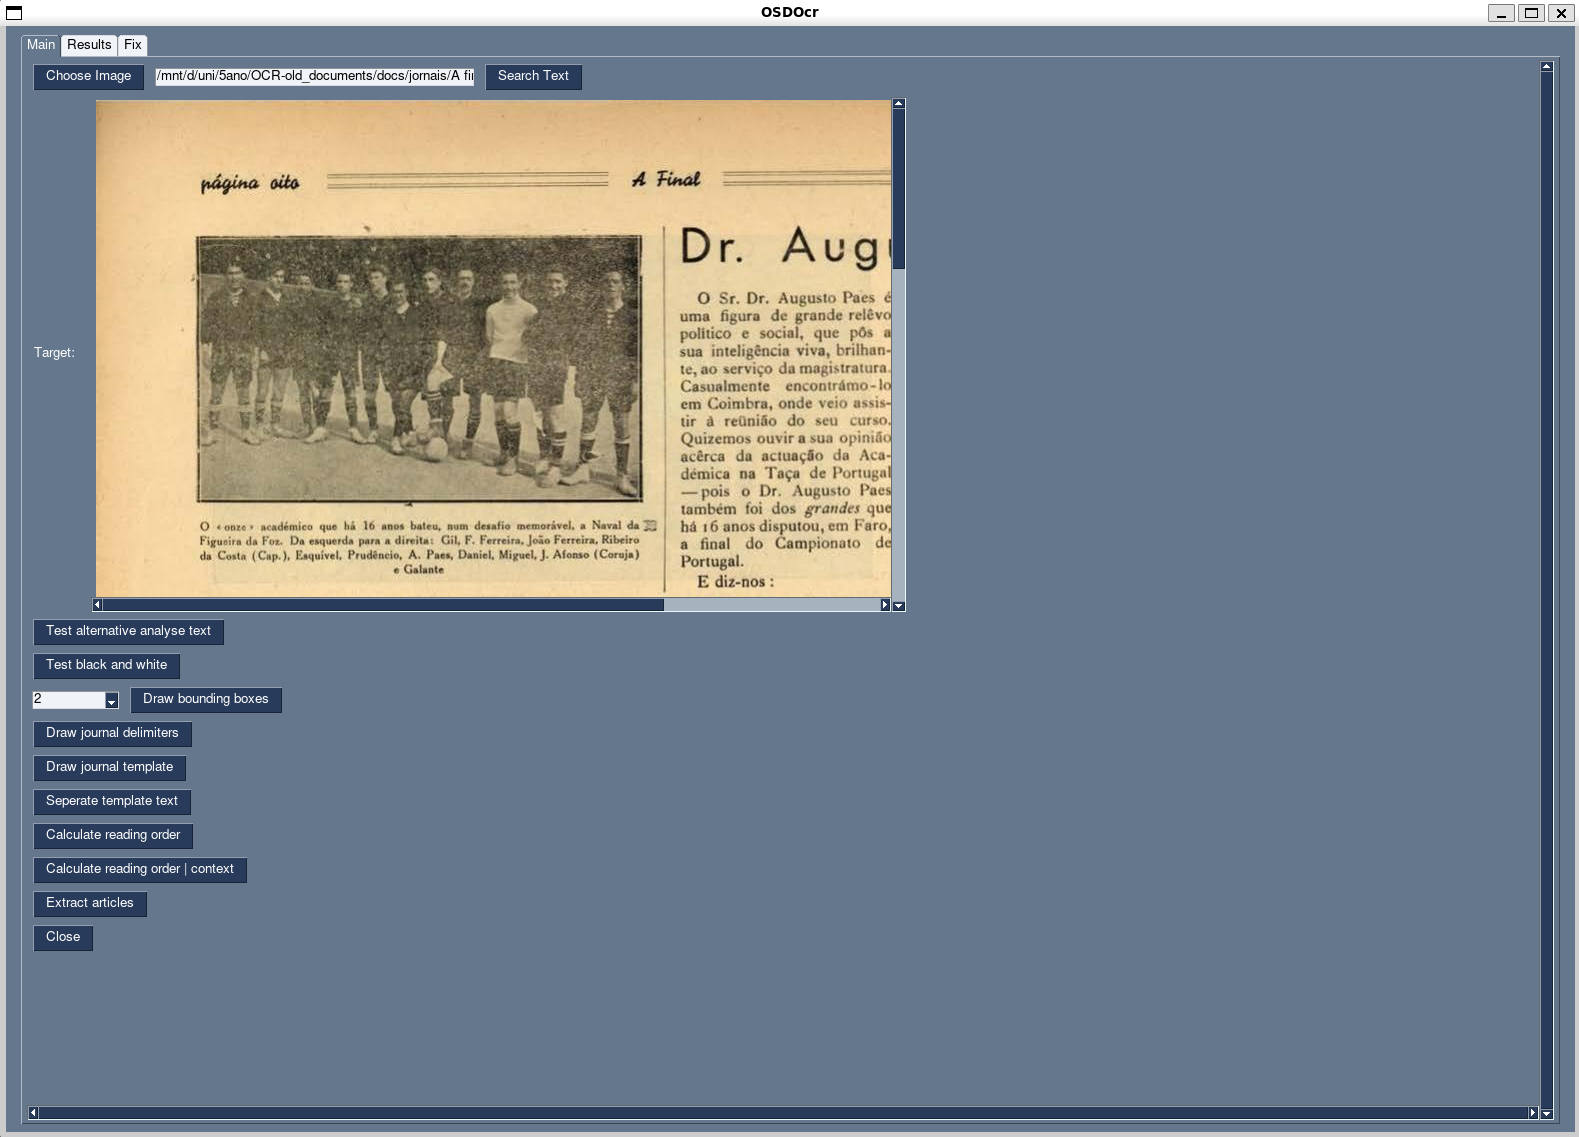
\includegraphics[width=1\textwidth]{images/implementacao/gui/gui_base.png}
%     \caption{Interface gráfica simples}
%     \label{fig:gui_base}
% \end{figure}
% 
% \subsubsection{Visualização de bounding boxes}
% 
% \begin{figure}[H]
%     \centering
%     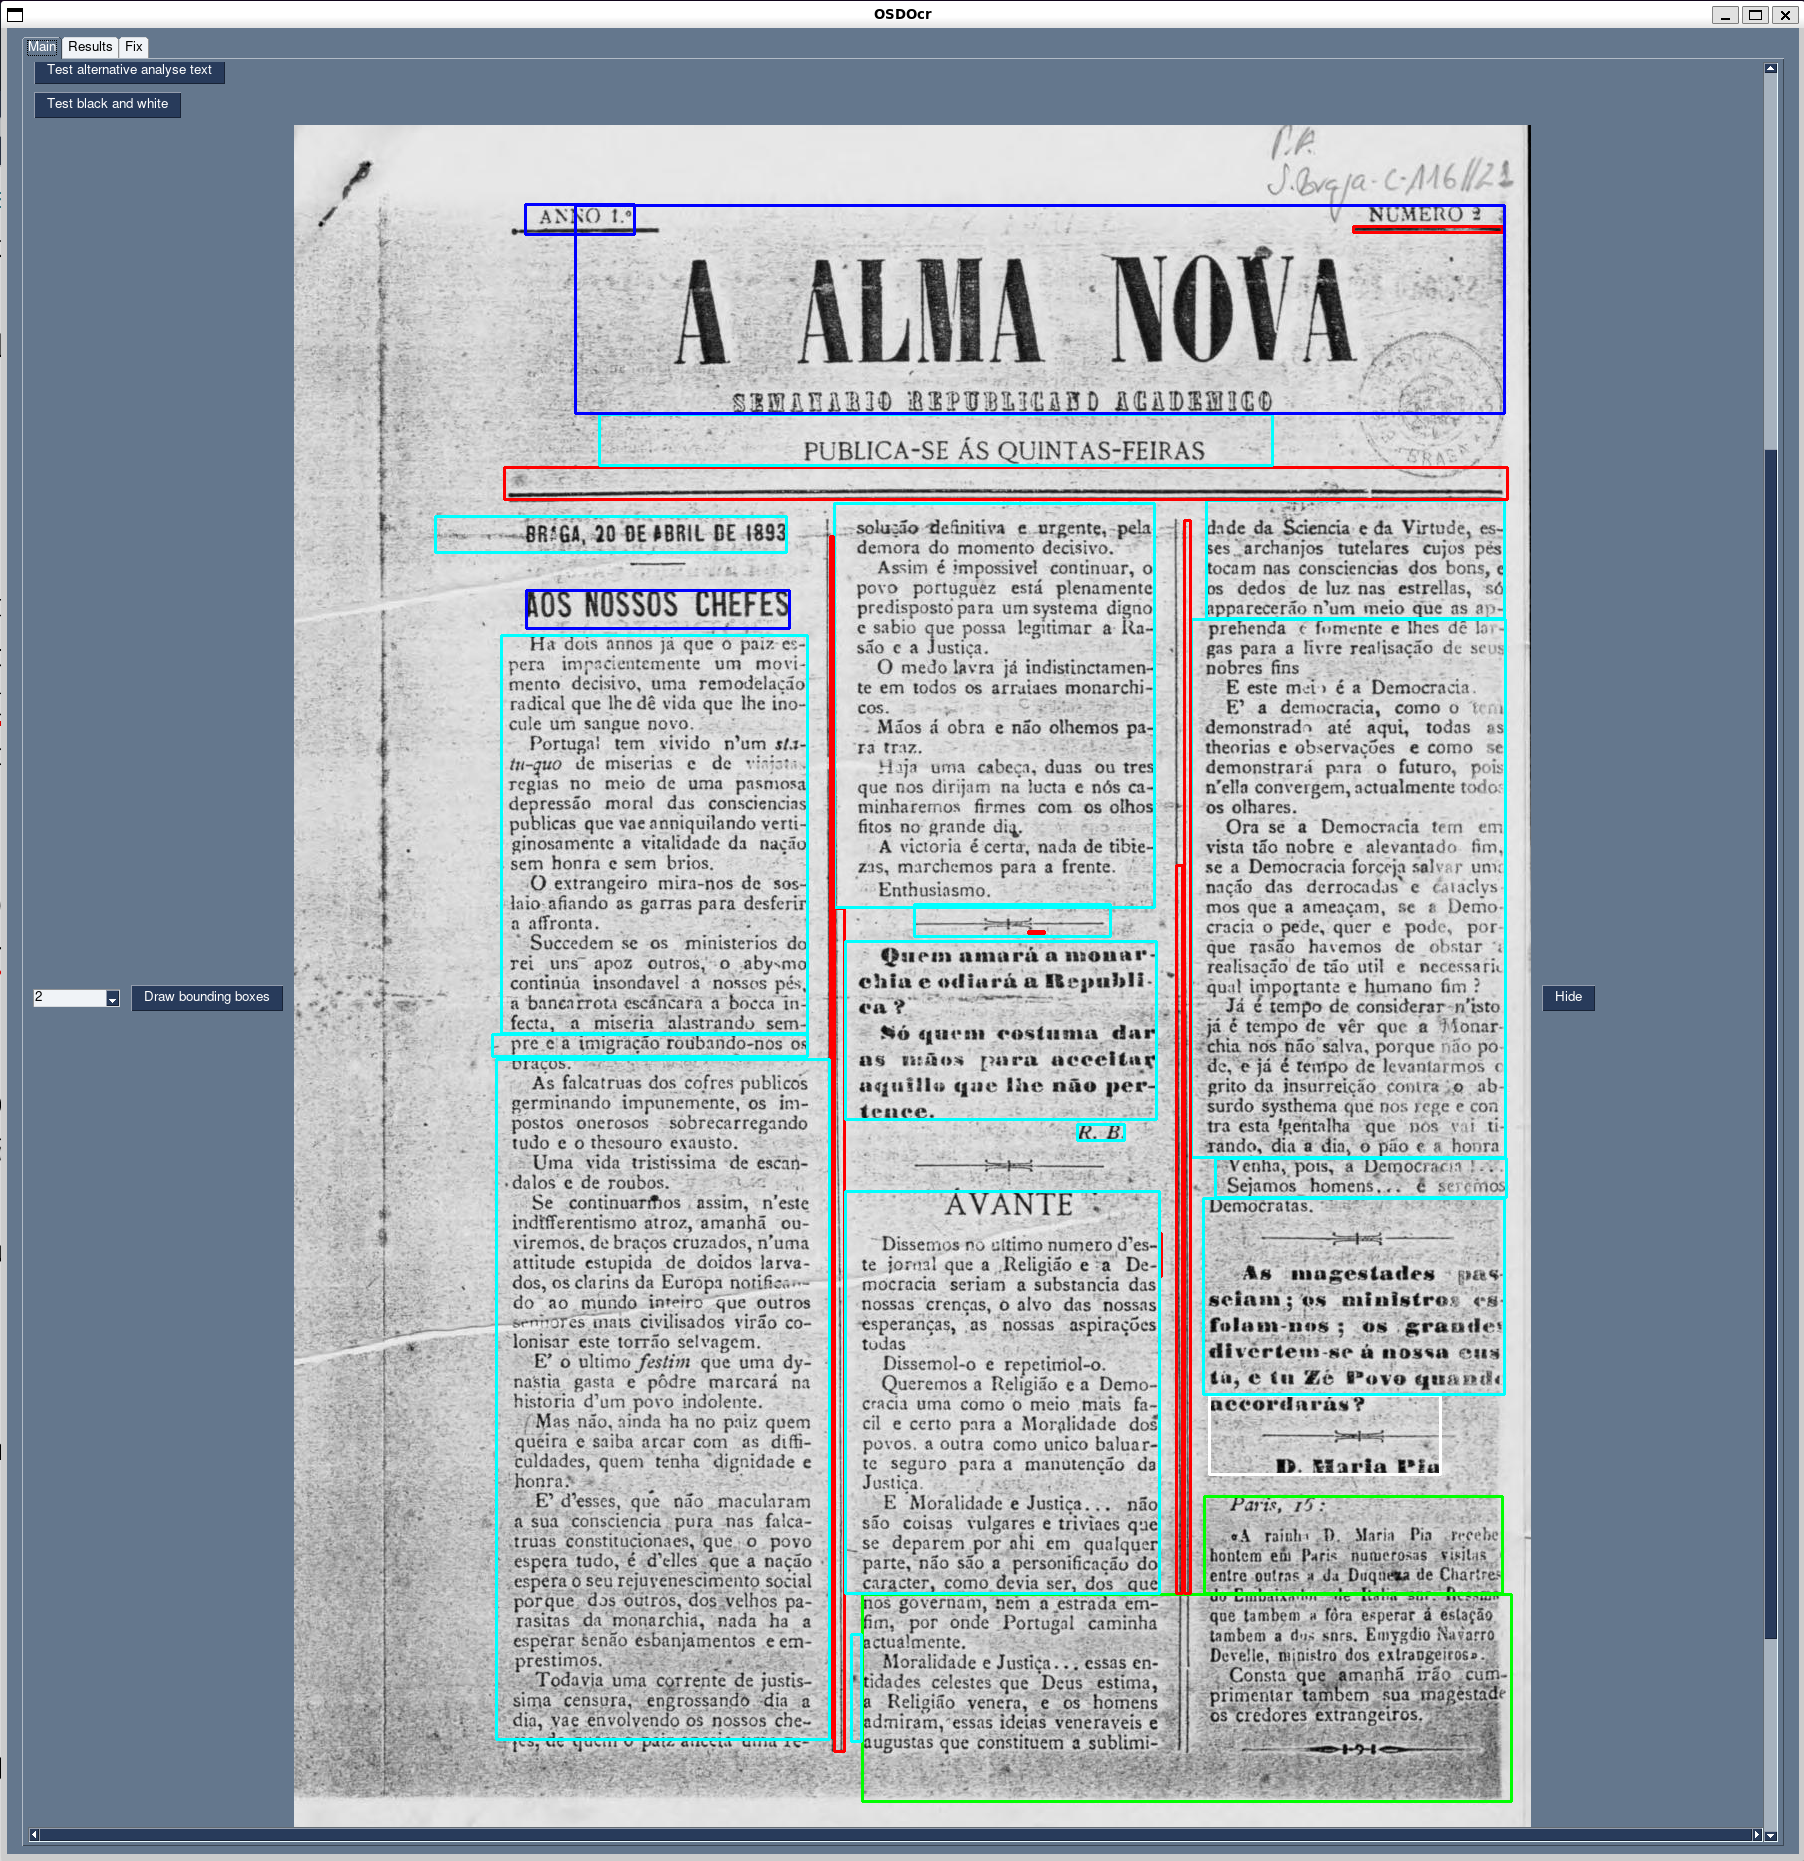
\includegraphics[width=1\textwidth]{images/implementacao/gui/gui_draw_bb.png}
%     \caption{Visualização dos blocos resultantes de OCR}
%     \label{fig:gui_draw_bb}
% \end{figure}
% 
% A visualização de blocos dispõe também de coloração diferente para os blocos de acordo com a sua categorização. Blocos título estão a azul escuro, texto a azul claro, delimitadores a vermelho, legendas a branco e o resto - imagens, outros - a verde.
% 
% \subsubsection{Cálculo de template de jornal}
% 
% \begin{figure}[H]
%     \centering
%     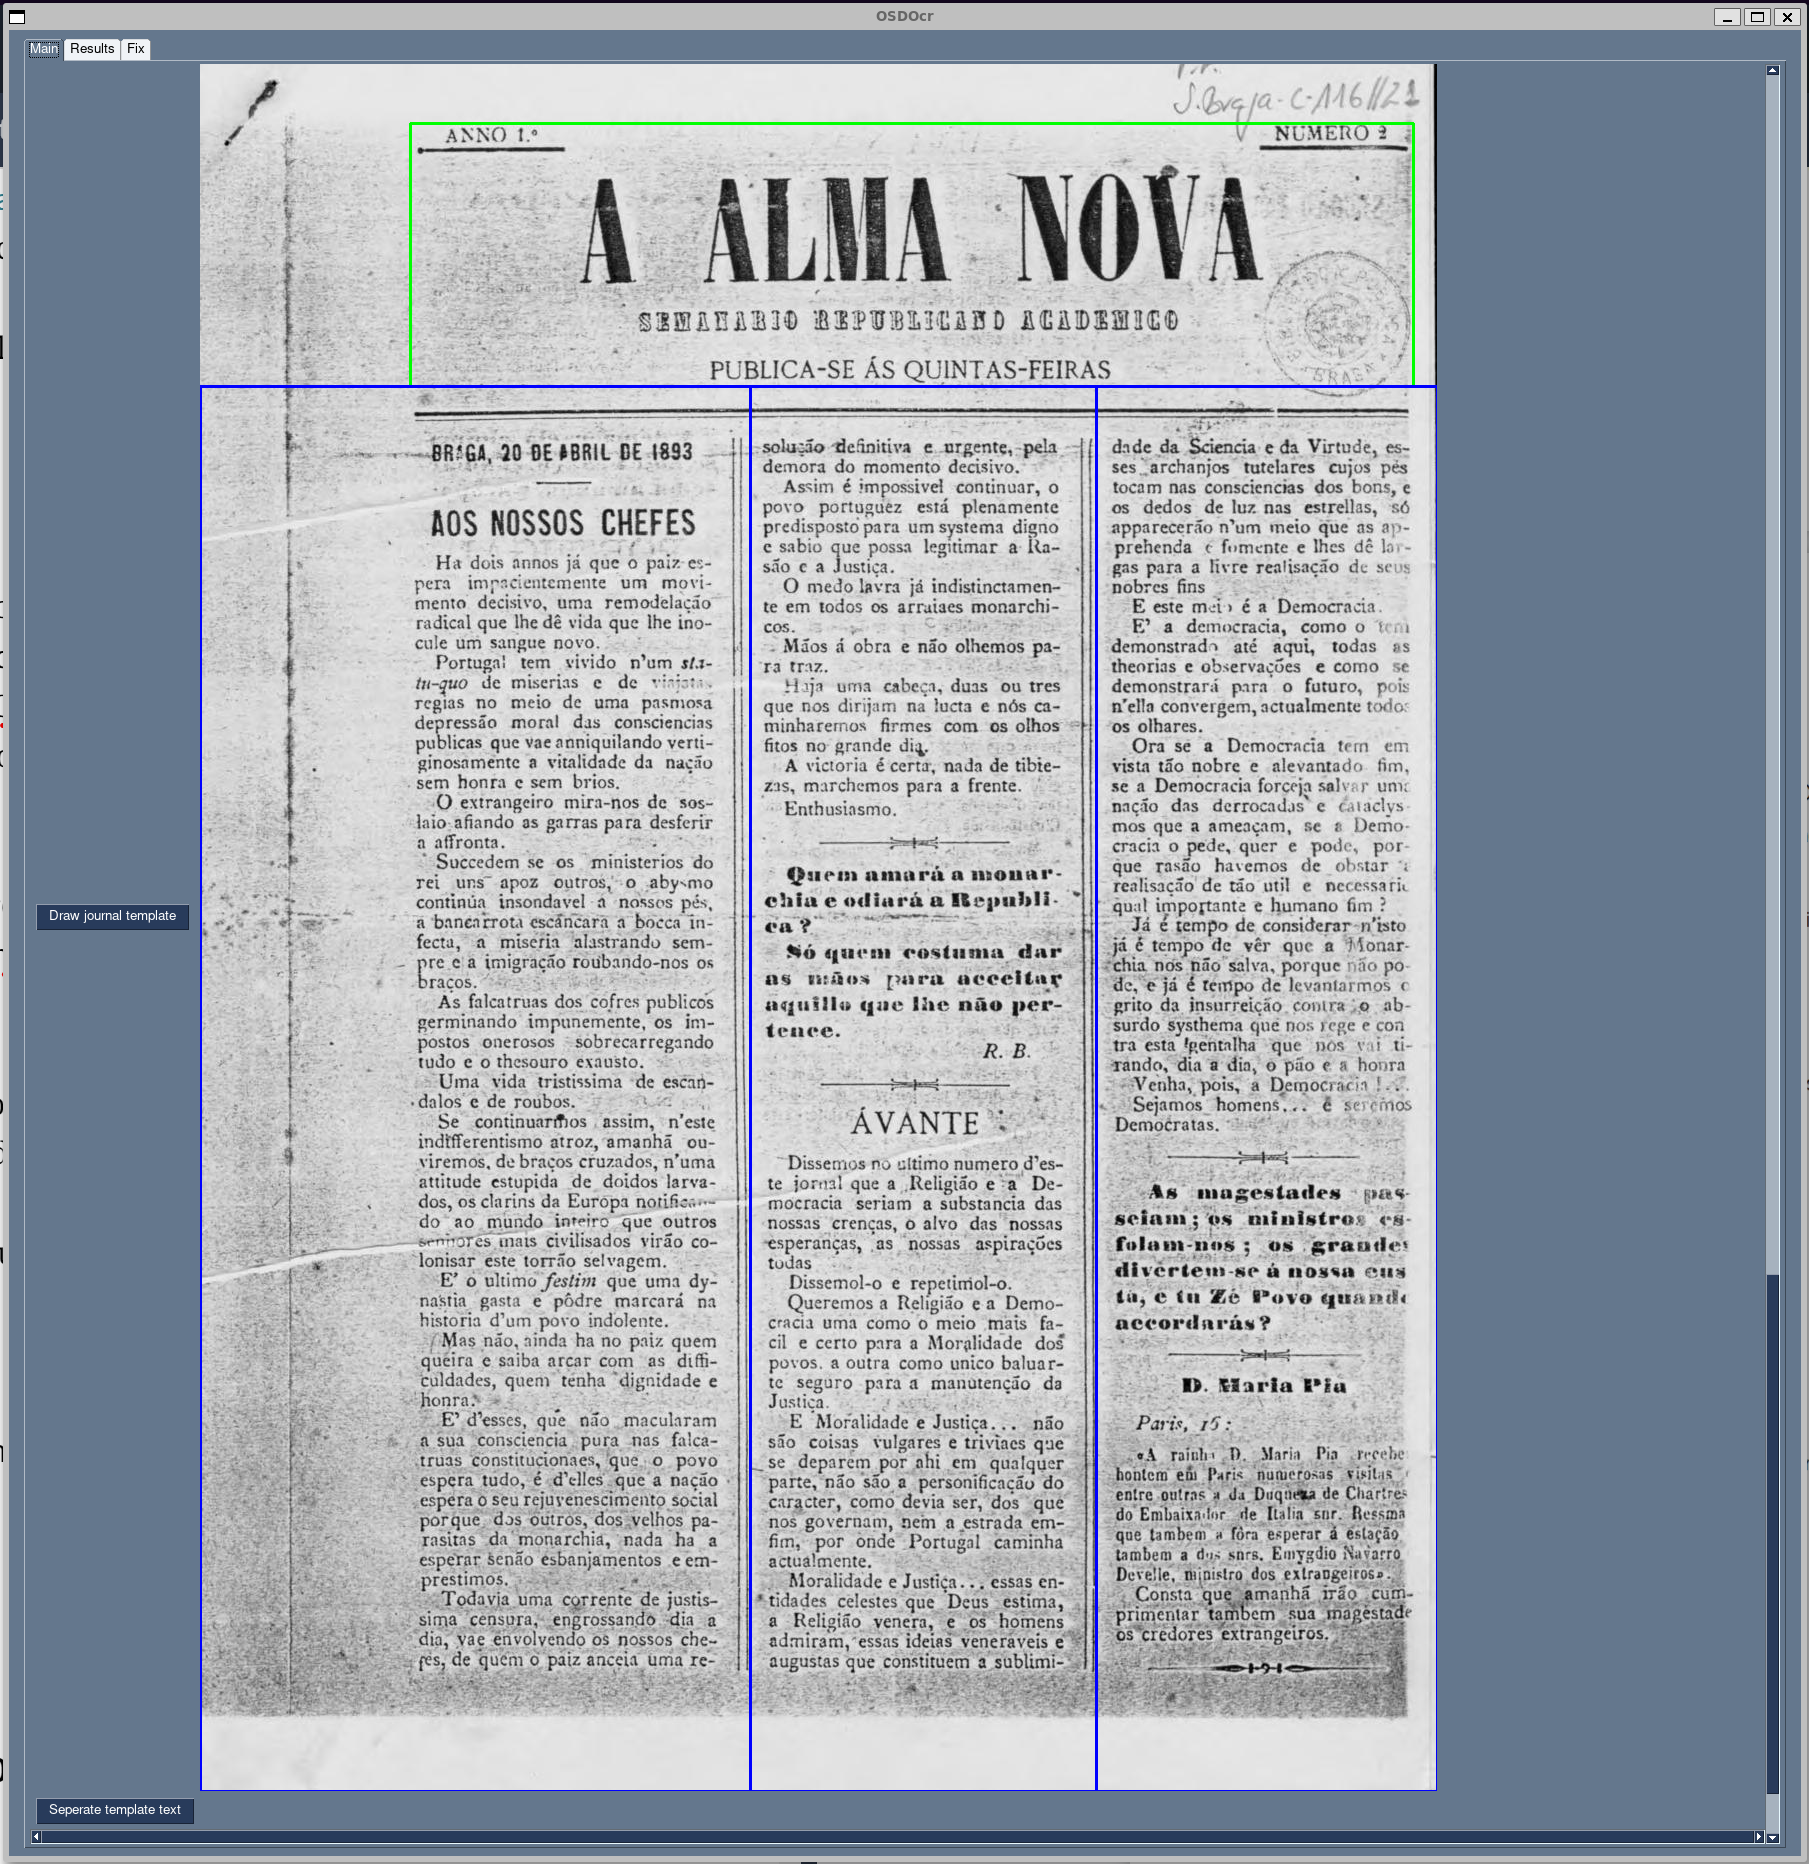
\includegraphics[width=1\textwidth]{images/implementacao/gui/gui_draw_template.png}
%     \caption{Visualização do cálculo do template de jornal}
%     \label{fig:gui_draw_template}
% \end{figure}
% 
% O cálculo de template é feito através da deteção e análise dos delimitadores dos resultados OCR. Áreas são depois calculadas de acordo com estes delimitadores e, como se pode ver no caso do Header (caixa a verde) da imagem \ref{fig:gui_draw_template}, a área é ajustada de acordo com as caixas com texto da respetiva área.
% 
% \subsubsection{Extração de artigos}
% 
% \begin{figure}[H]
%     \centering
%     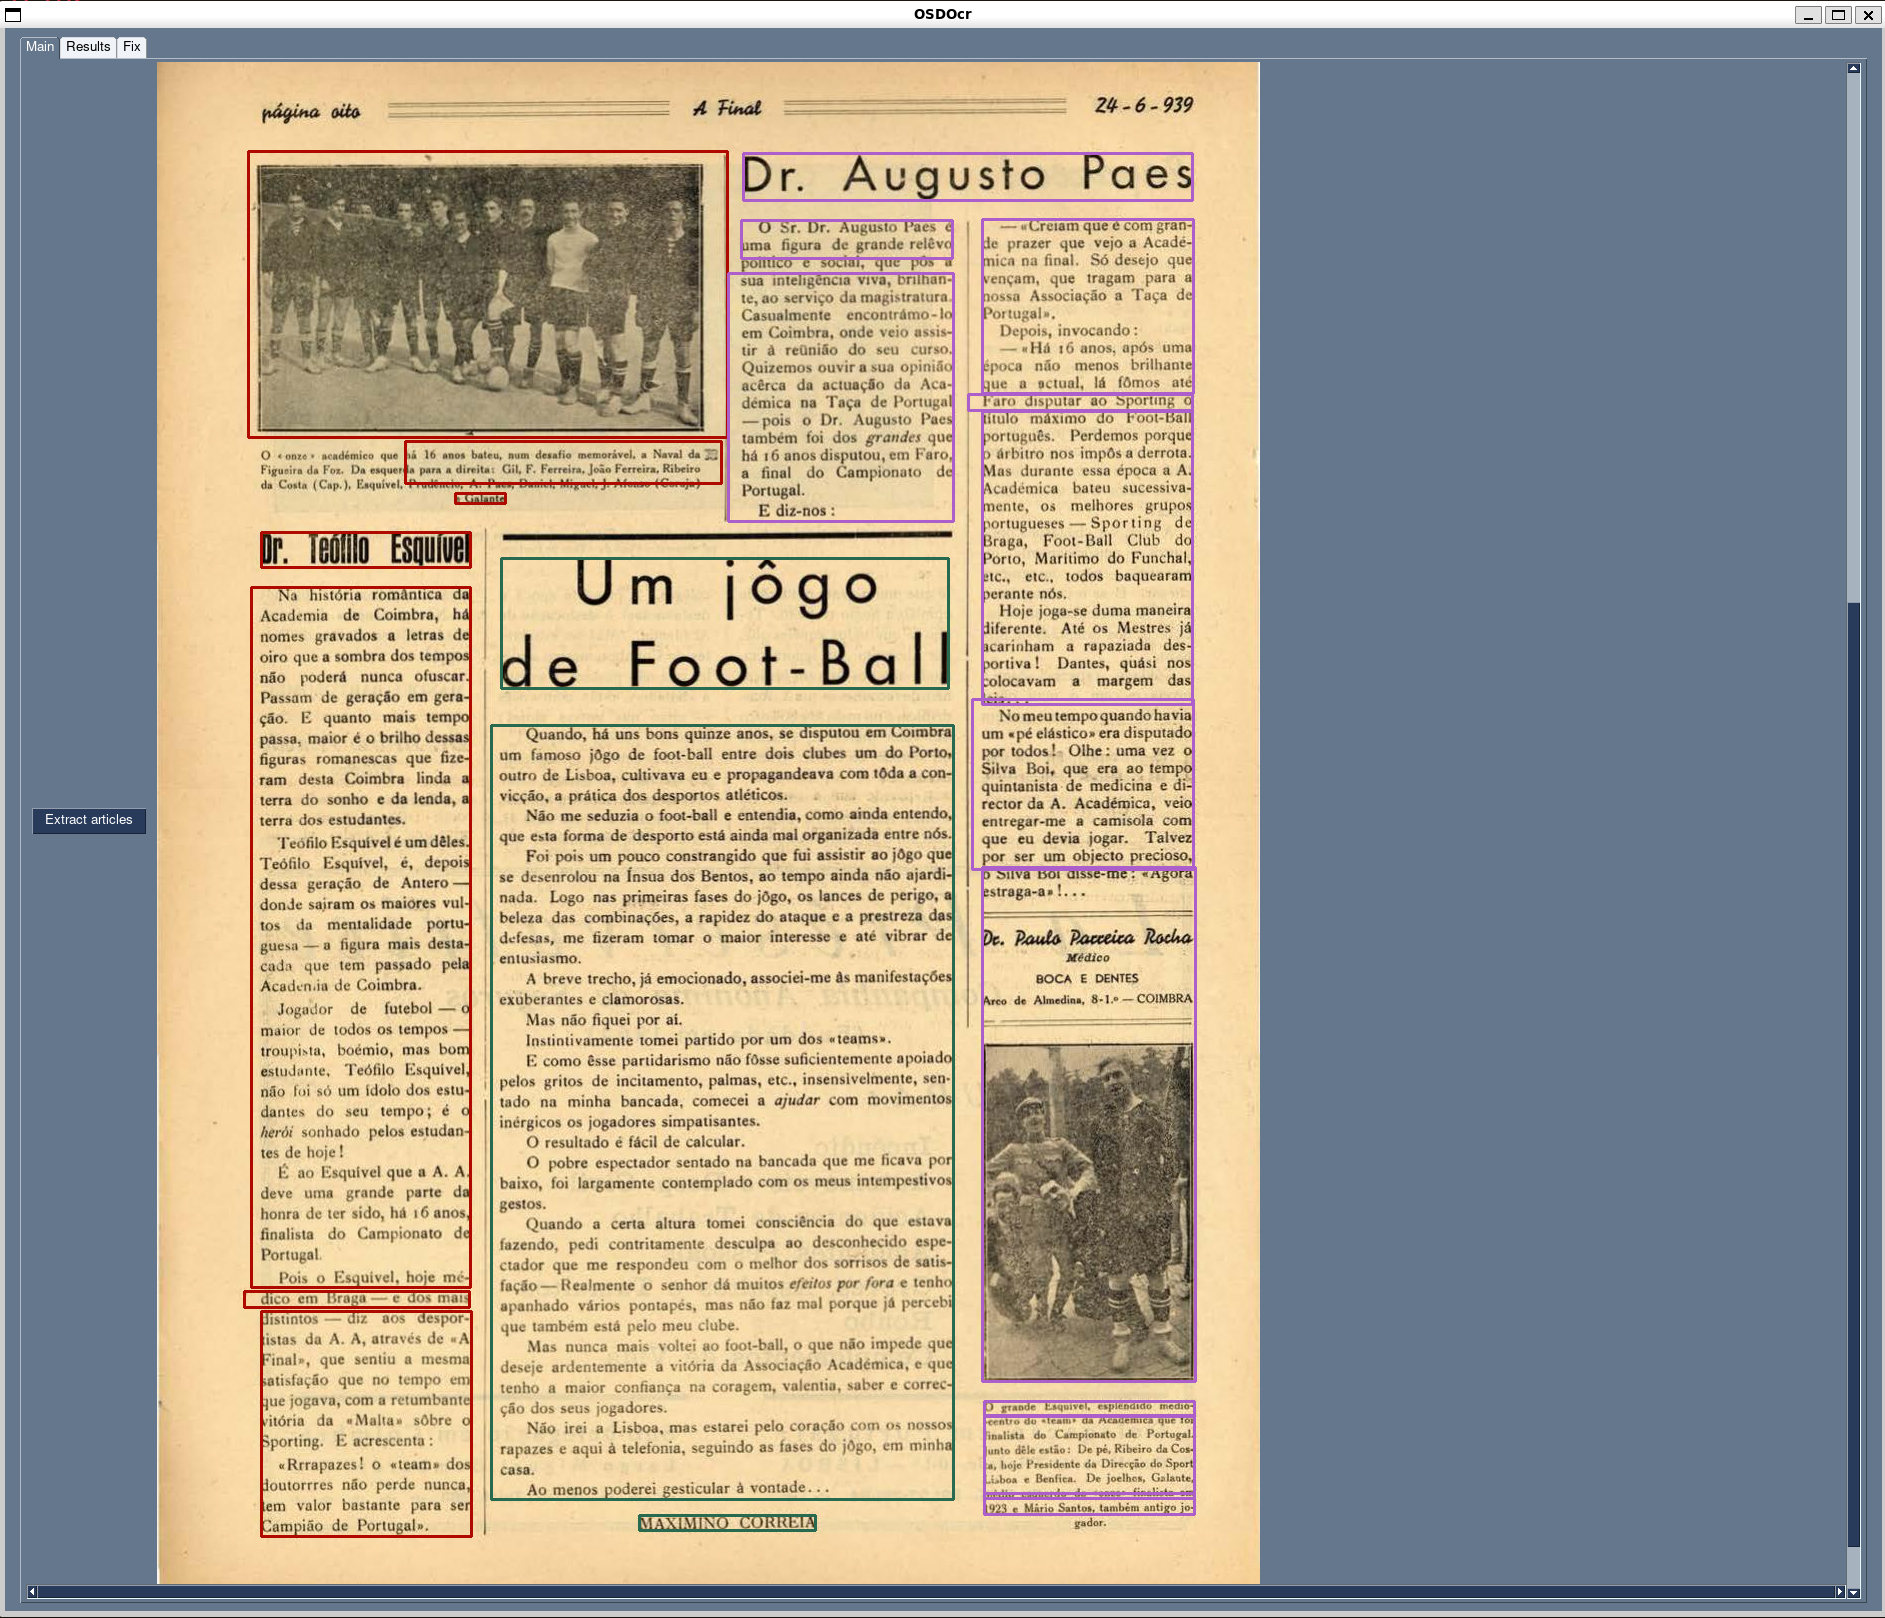
\includegraphics[width=1\textwidth]{images/implementacao/gui/gui_draw_articles.png}
%     \caption{Visualização dos artigos extraídos}
%     \label{fig:gui_draw_article}
% \end{figure}
% 
% Neste caso, os artigos são calculados e posteriormente escolhidas cores distintas para realçar cada um destes. Os artigos são representados pelo conjunto de blocos que foram agrupados como sendo um dado artigo.
% 
% \subsubsection{Limpeza de bounding boxes}
% 
% \begin{figure}[H]
%     \centering
%     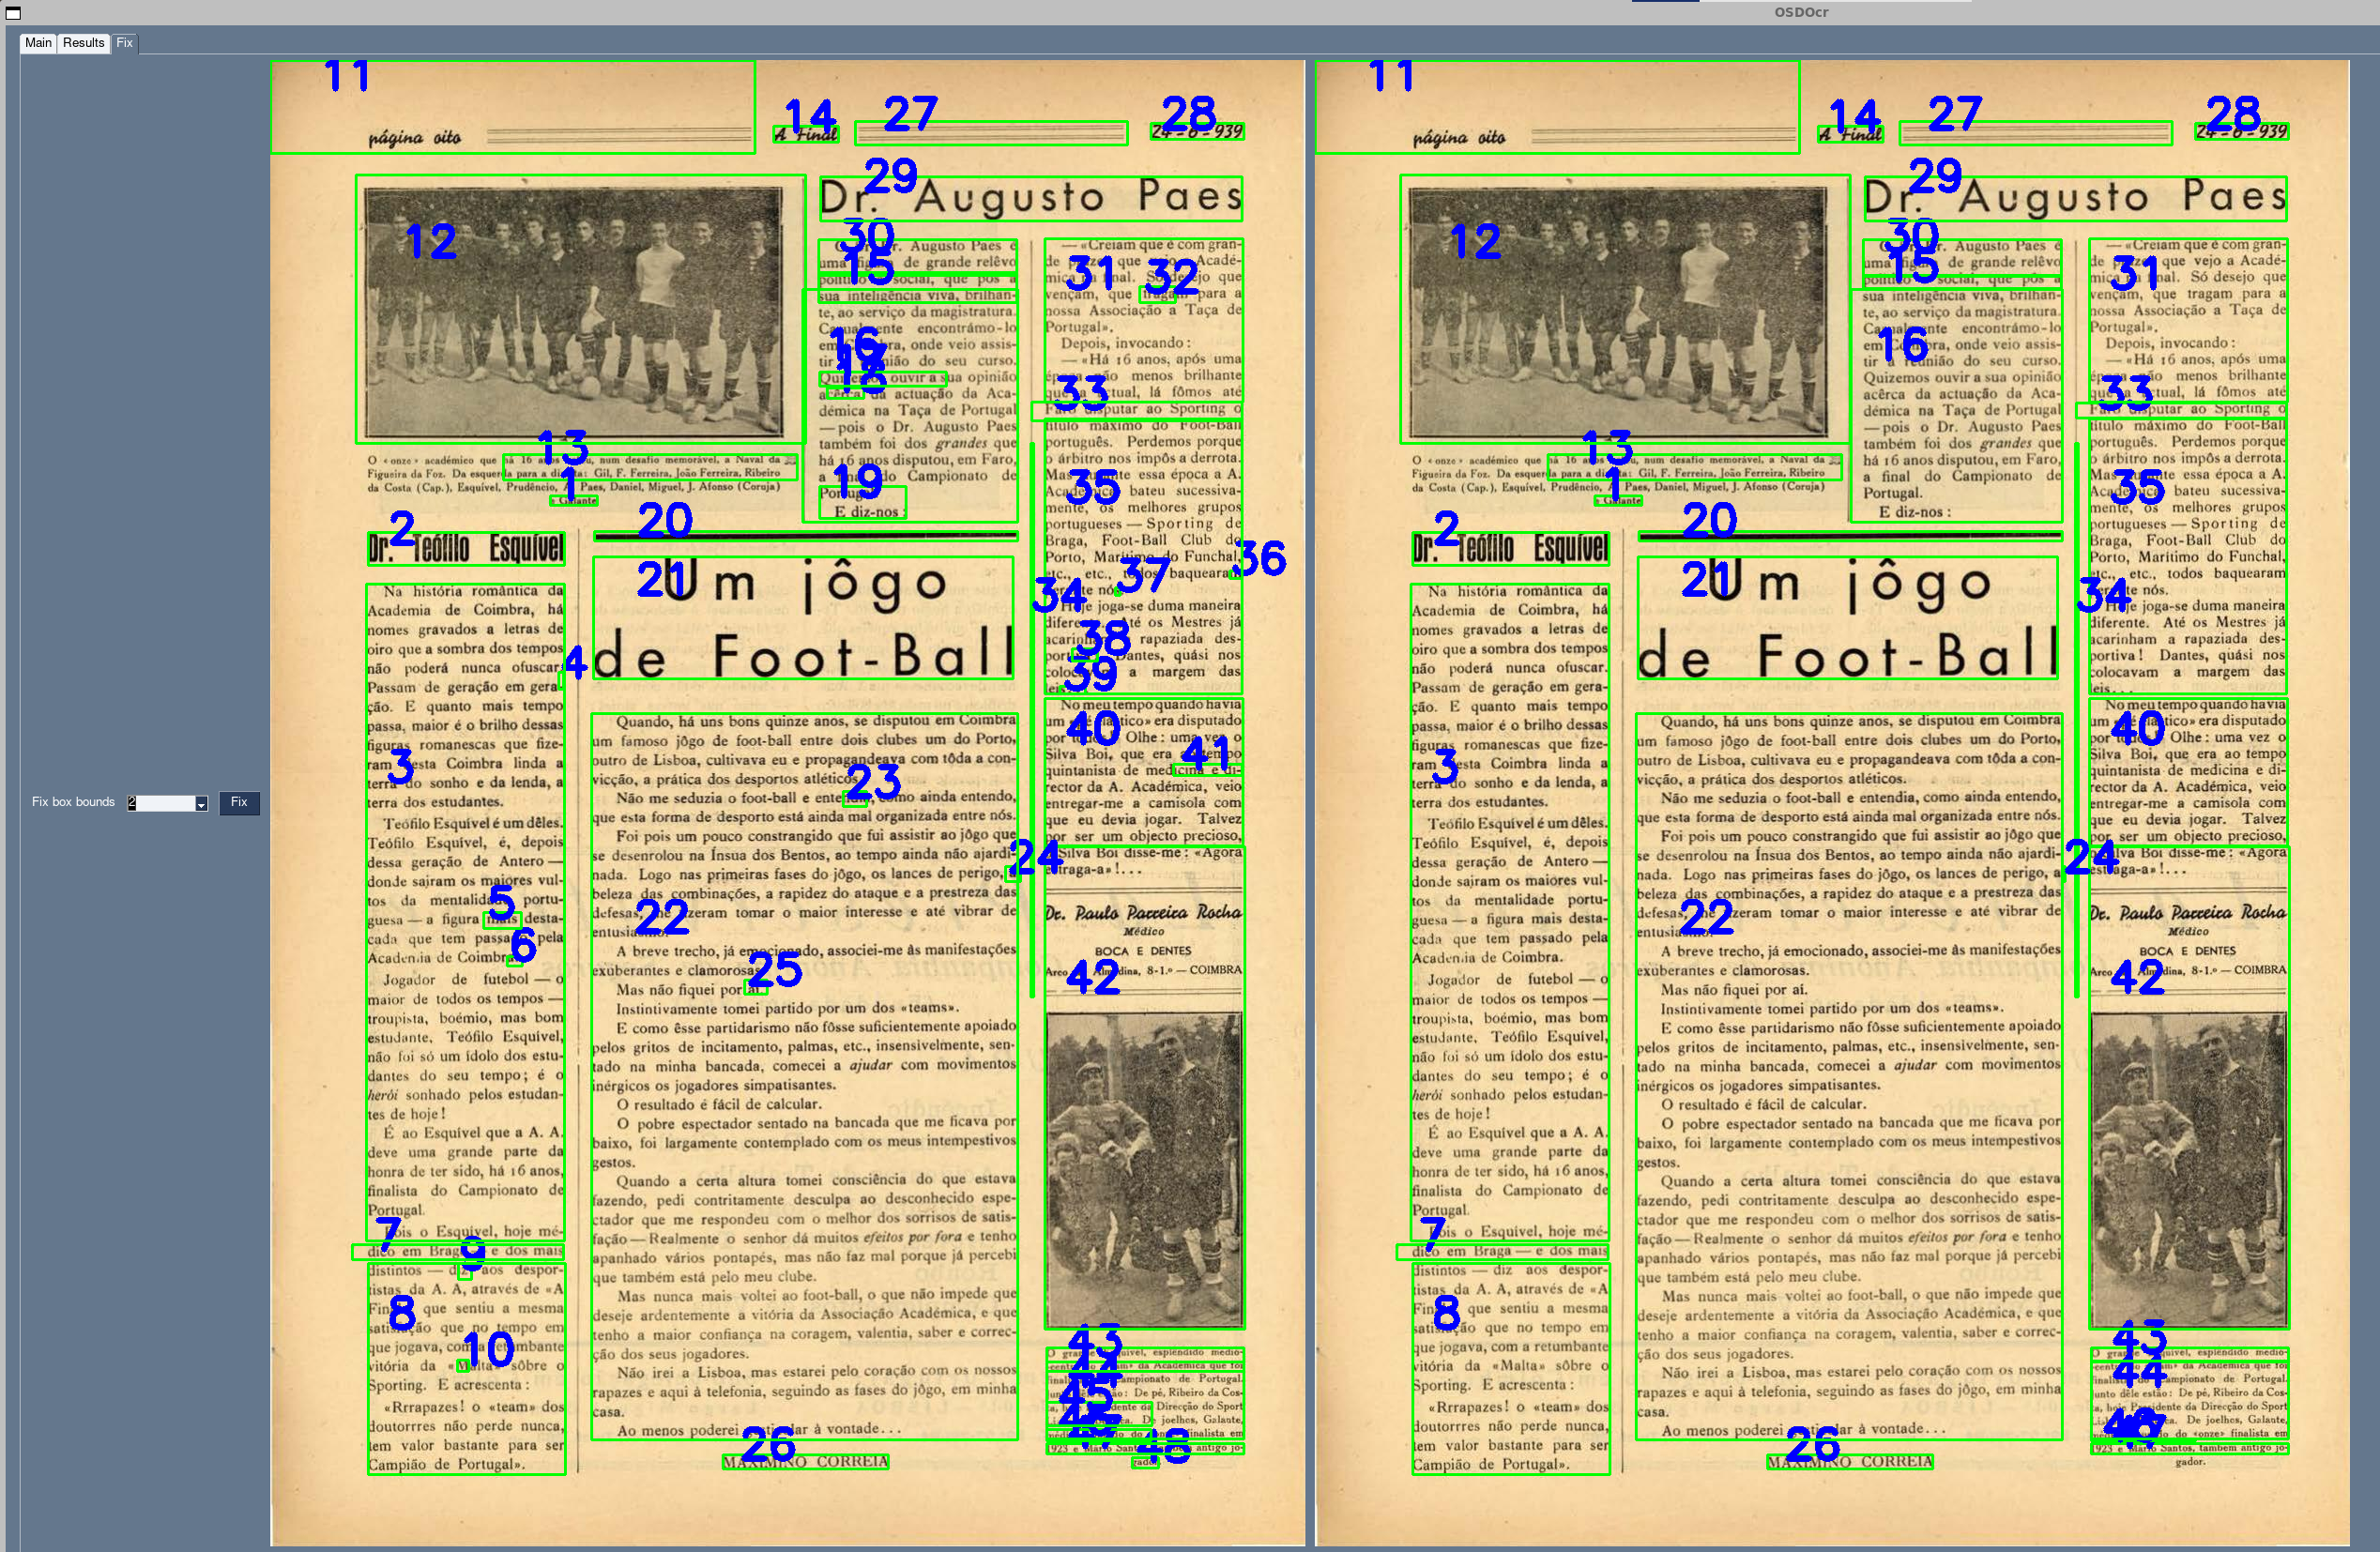
\includegraphics[width=1\textwidth]{images/implementacao/gui/gui_fix_blocks.png}
%     \caption{Visualização da limpeza de blocos}
%     \label{fig:gui_fix_bb}
% \end{figure}
% 
% Para facilitar a deteção das diferenças entre o antes e depois da limpeza, os dois estados são postos lado a lado e os blocos são identificados, mantendo a mesma identificação após a limpeza. 





\chapter{Aplicações}

Aplicação do resultado principal (exemplos e casos de estudo)

\section{Introdução}

\section{Sumário}
\chapter{Conclusões e trabalho futuro}
\label{cap_conclusao}

Neste capítulo será feito um sumário do trabalho e estudo realizado, tiradas conclusões sobre o projeto concebido, e uma introspeção sobre perspetivas de trabalho futuro.

\section{O Trabalho}

A dissertação propôs como seu objetivo global, a criação de uma solução que pode-se ser acoplada ao processo de reconhecimento ótico de caracteres, tanto antes e depois deste, para a melhoria dos seus resultados. 

Através do estudo do problema, focado essencialmente em jornais antigos - devido à sua mutabilidade de estrutura e geral estado deteriorado que afetam a transcrição máquina -, foi possível delimitar a solução em componentes distintas. Estas foram : um Toolkit ou conjunto de métodos que permitam realizar transformações, sobretudo nos resultados de OCR mas também incluindo processamento de imagem e texto, em via de reduzir erros na transcrição e facilitar a sua manipulação e análise dos resultados OCR; uma pipeline, estrutura semelhante à maioria de problemas que abordam este tema, e que permite a aplicação e consequente validação do Toolkit; um editor gráfico de resultados OCR que disponibilize um meio de manipulação de resultados OCR facilitada, assim como depuração facilitada - pelo seu aspeto visual - das duas anteriores componentes.

Essas 3 componentes tiveram em comum a necessidade de analisar e manipular resultados OCR, o que resultou na criação de uma estrutura universal para estes, OCR Tree.

Discutida a implementação deste modelo e componentes, foram também analisados os seus resultados quando aplicados em diferentes contextos, com especial atenção para a pipeline, sendo esta a mais permissiva de métricas objetivas.

O código desenvolvido e ficheiros de resultados pode ser encontrado em:
\begin{itemize}
	\item \href{https://github.com/brazafonso/OCR-old_documents}{Repositório principal}
	\item \href{https://github.com/brazafonso/document_image_processing}{Repositório auxiliar com métodos para tratamento de imagem}
	\item \href{https://drive.google.com/drive/u/0/folders/1DW-AIuSxjEyv6ioq7jX8P1xruy03Sxo9}{Ficheiros de resultados}
\end{itemize}



\section{Conclusões}

Concluído o trabalho, é possível comparar a sua visão inicial do estado atual. Num primeiro desenho do projeto, apenas se expectava a implementação de um conjunto de métodos independentes e, incontornavelmente, o modelo OCR Tree.

Este conjunto de ferramentas sucedeu na criação de uma estrutura de dados complexa, mas de compreensiva manipulação e análise, tendo sido esta área o seu ponto forte. Além disso, na área de tratamento e análise de imagem, ferramentas de correção de anomalias de imagem e identificação de elementos de documento como delimitadores e colunas, que foram aplicados nas outras partes da solução. Porém, com o desenvolvimento desta componente entendeu-se a necessidade de um ambiente de teste da mesma. 

Daqui nasce a pipeline, nova componente que, embora já desde inícios do trabalho pensada, inevitavelmente obrigou a divisão dos esforços na primeira componente, tendo essa pecado principalmente em aspetos de tratamento de texto.
A pipeline, como aplicação do Toolkit, foi também aproveitada para abranger aspetos que este não iria abordar, como o upscaling de imagem. Utilizando a pipeline, é possível a observação direta do efeito do Toolkit na transcrição máquina, permitindo ainda, métricas objetivas através do módulo de validação nesta implementada.

Esta foi testada utilizando um conjunto de casos de teste - utilizando o próprio módulo de validação da pipeline- , os quais foram executados com diferentes configurações de características fundamentalmente diferentes, não adaptadas para nenhum caso em particular. Concluiu-se a partir destes teste que a pipeline é mais útil quando a configuração fornecida é adaptada aos problemas de um documento, sendo que não obteve na globalidade resultados notórios utilizando as configurações generalizadas. Por outro lado, em casos pontuais certas configurações, mesmo generalizadas, obtiveram melhorias consideráveis em relação a OCR base, demonstrando-se o seu potencial. Além disso, notou-se a utilidade da secção de pós processamento para diminuição da complexidade dos resultados OCR, e a oportunidade que uma evolução no módulo de tratamento de texto poderia trazer para o output final.

Na presença de questões mais minuciosas que a pipeline não foi capaz de lidar, como: ordens de leitura muito complexos, trechos de texto demasiado danificados para transcrição automática, segmentação insatisfatória do motor OCR; e também a dificuldade em visualizar o estado da OCR Tree durante as diferentes etapas da Pipeline ou manipulações pelo Toolkit, gerou-se a oportunidade de incluir um editor visual. Este foi a última e mais tardia componente a ser incluída na solução mas, possivelmente, a mais útil. Esta componente permitiu uma suavização no uso da OCR Tree que, consideravelmente, habilitou a compensação de problemas ignorados ou não totalmente tratados pela Pipeline, assim como a potencialização do Toolkit, fazendo uso de partes dele até então desusadas. Adicionalmente, este meio de visualizar a manipulação permitida pelas anteriores componentes, permitiu mais facilmente detetar defeitos nelas ou possíveis melhorias, recursivamente melhorando-se ao simplificar o refinamento delas.

O compilado de todas as componentes foi essencial para um aprofundamento do conhecimento sobre a área de pré, e particularmente, pós processamento de OCR, modularização de soluções e, no caso do Editor, o trabalho sobre interfaces gráficas e editor de modelos.



\section{Perspetiva de trabalho futuro}

Apesar de satisfeito e enriquecido com a realização do projeto, seria ingénuo ignorar os refinamentos que este poderia ser sujeito. 

Como já referido, a área em que o Toolkit mais tem espaço para enriquecer trata-se do tratamento de texto, mais especificamente no ato de criação de output. Tal, como os tempos têm mostrado haver um maior potencial, daria-se provavelmente na exploração de Large Language Models para a realização de correções de texto, que possivelmente também poderiam permitir a restauração de texto não detetado/transcrito. Naturalmente, heurísticas mais determinísticas para tratamento de texto também seriam bem-vindas, como, por exemplo, as técnicas exploradas no estado da arte, de correção de palavras fazendo uso de léxicos conhecidos.

Do mesmo modo, embora neste caso já levemente explorado, o processamento de imagem fazendo uso de inteligência artificial seria inevitável, nomeadamente para: correção de distorções de imagens como curvaturas do texto ou inclinações internas; restauro de texto. De forma mais complexa, e como também foi mencionado no estado da arte, acoplar a visão máquina com os mecanismos criados para cálculo de ordem de leitura, categorização de texto e isolamento de artigos tem o potencial de aumentar a adaptabilidade destes. As restrições temporais e de recursos não permitiram porém divergência neste sentido, podendo por si só este ramo tornar-se num projeto único.

A estrutura OCR Tree poderia ser tornada mais 'universal' para OCR relaxando a responsabilidade dos níveis de blocos, visto pressupor atualmente na maioria dos cenários que o nível 2 é representativo de um bloco como um todo, e o 5 como o local de texto. Por exemplo, na procura de texto, poderia ser possível incluir texto em blocos superiores, reduzindo a necessidade de sempre iterar às folhas para o obter; ou no caso de análise de texto, utilizar como base o nível fornecido ao invés de assumir os níveis 4 (linha) e 5 (palavra) como essenciais.

O módulo de output teria bem-vinda a conversão para um formato que mantivesse mais fielmente a estrutura original do documento, como pdf ou html. A existência de conversores de hocr para estes terá diminuído a sua prioridade.

Como discutido durante a análise de resultados, o estudo de uma pipeline auto configurável seria interessante para a criação de uma solução adaptável a documentos de diferentes características. 


Por último, a exploração de diferentes motores OCR seria relevante para prova da potencialidade da OCR Tree como módulo para resultados OCR, e possibilitando mais uso de todas as componentes da solução.


		
\chapter{Planeamento}

\section{Atividades}

\newacronym{rpd}{RPD}{Relatório de Pré-Dissertação}
\newacronym{eda}{EA}{Estado da Arte}

\begin{table}[H]
\begin{center}
\begin{tabular}{| c | c | c | c | c | c | c | c | c | c | c |}
\hline
\textbf{Tarefa} & \textbf{Out} & \textbf{Nov} & \textbf{Dez} & \textbf{Jan} & \textbf{Fev} & \textbf{Mar} & \textbf{Abr} & \textbf{Mai} & \textbf{Jun} & \textbf{Jul}\\
\hline
\textit{Background} e \acrshort{eda} & $\bullet$ & $\bullet$ & $\bullet$ & & & & & & & \\
\hline
Preparação do \acrshort{rpd} & & $\bullet$ & $\bullet$ & $\bullet$ & & & & & & \\
\hline
Contribuição & & & &$\bullet$ &$\bullet$ &$\bullet$ &$\bullet$ &$\bullet$ &$\bullet$ & \\
\hline
Escrita & & & & & & & $\bullet$ & $\bullet$ & $\bullet$ & $\bullet$ \\
\hline
\end{tabular}
\end{center}
\caption{Plano de atividades.}
\end{table}


\renewcommand{\baselinestretch}{1}
\bibliographystyle{plainnat}
\bibliography{dissertation}
\printindex

\appendix
\renewcommand\chaptername{Apêndice}

\part{Apêndices}

\chapter{Trabalho de apoio}
Resultados auxiliares.
\chapter{Detalhes dos resultados}
Detalhes de resultados cuja extensão comprometeria a legibilidade do texto principal.
\chapter{Listings}
Se for o caso.
\chapter{Ferramentas}

\begin{itemize}
	\item \href{https://github.com/tesseract-ocr/tesseract}{Tesseract} : motor OCR utilizado
	
	\item \href{https://www.pysimplegui.com}{PySimpleGui} : base para criação de interface OSDOCR Editor
	
	\item \href{https://matplotlib.org}{Matplotlib} : base para canvas de interação de OSDOCR Editor
	
	\item \href{https://github.com/nagadomi/waifu2x}{Modelos de upscaling de imagem - waifu2x}
	
	\item \href{https://github.com/Fediory/HVI-CIDNet}{Modelos de melhoria de iluminação de documentos - HVI-CIDNet}
	
\end{itemize}

\pagestyle{empty}
\cleartoevenpage
\null
\thispagestyle{empty}
\pagecolor{PANTONECoolGray7C}
\afterpage{\nopagecolor}
\newpage

\begin{backcover}
\thispagestyle{empty}{~\vfill
\noindent
Coloque aqui informação sobre financiamento, projeto FCT, etc. em que o trabalho se enquadra. Deixe em branco caso contrário.
\vfill ~}
\end{backcover}



\end{document}
